\documentclass[9pt]{article}

\usepackage[super,sort&compress,comma]{natbib}
\usepackage[left=1.5cm, right=1.5cm, top=1.785cm,
bottom=2.0cm]{geometry}
\usepackage[english]{babel}
\usepackage[T1]{fontenc}
\usepackage{hyperref}
\usepackage{graphicx}
\graphicspath{{./figures}{../figures}}
\usepackage{xcolor}

\usepackage{graphicx}
\usepackage{booktabs}
\usepackage{multirow}

%\usepackage{epstopdf}
\usepackage{epstopdf}


\renewcommand{\thepage}{S\arabic{page}}
\renewcommand{\thesection}{S\arabic{section}}
\renewcommand{\thetable}{S\arabic{table}}
\renewcommand{\thefigure}{S\arabic{figure}}

\begin{document}

\noindent\LARGE{\textbf{Size Matters: Free-energy Calculations of Amino Acid Adsorption over Prisitine Graphene. \\ Supplementary material.}} \\
\vspace{0.1cm} %& \vspace{0.1cm} \\

\noindent\large{Mateo Barria-Urenda, Alvaro Ruiz-Fernandez, Carlos Gonzalez, Chris Oostenbrink and Jose Antonio Garate}

\tableofcontents

\newpage

\section{Potentials of Mean Force}
\subsection{Adsorption over graphene}

\begin{figure}[hbtp]
    \centering
    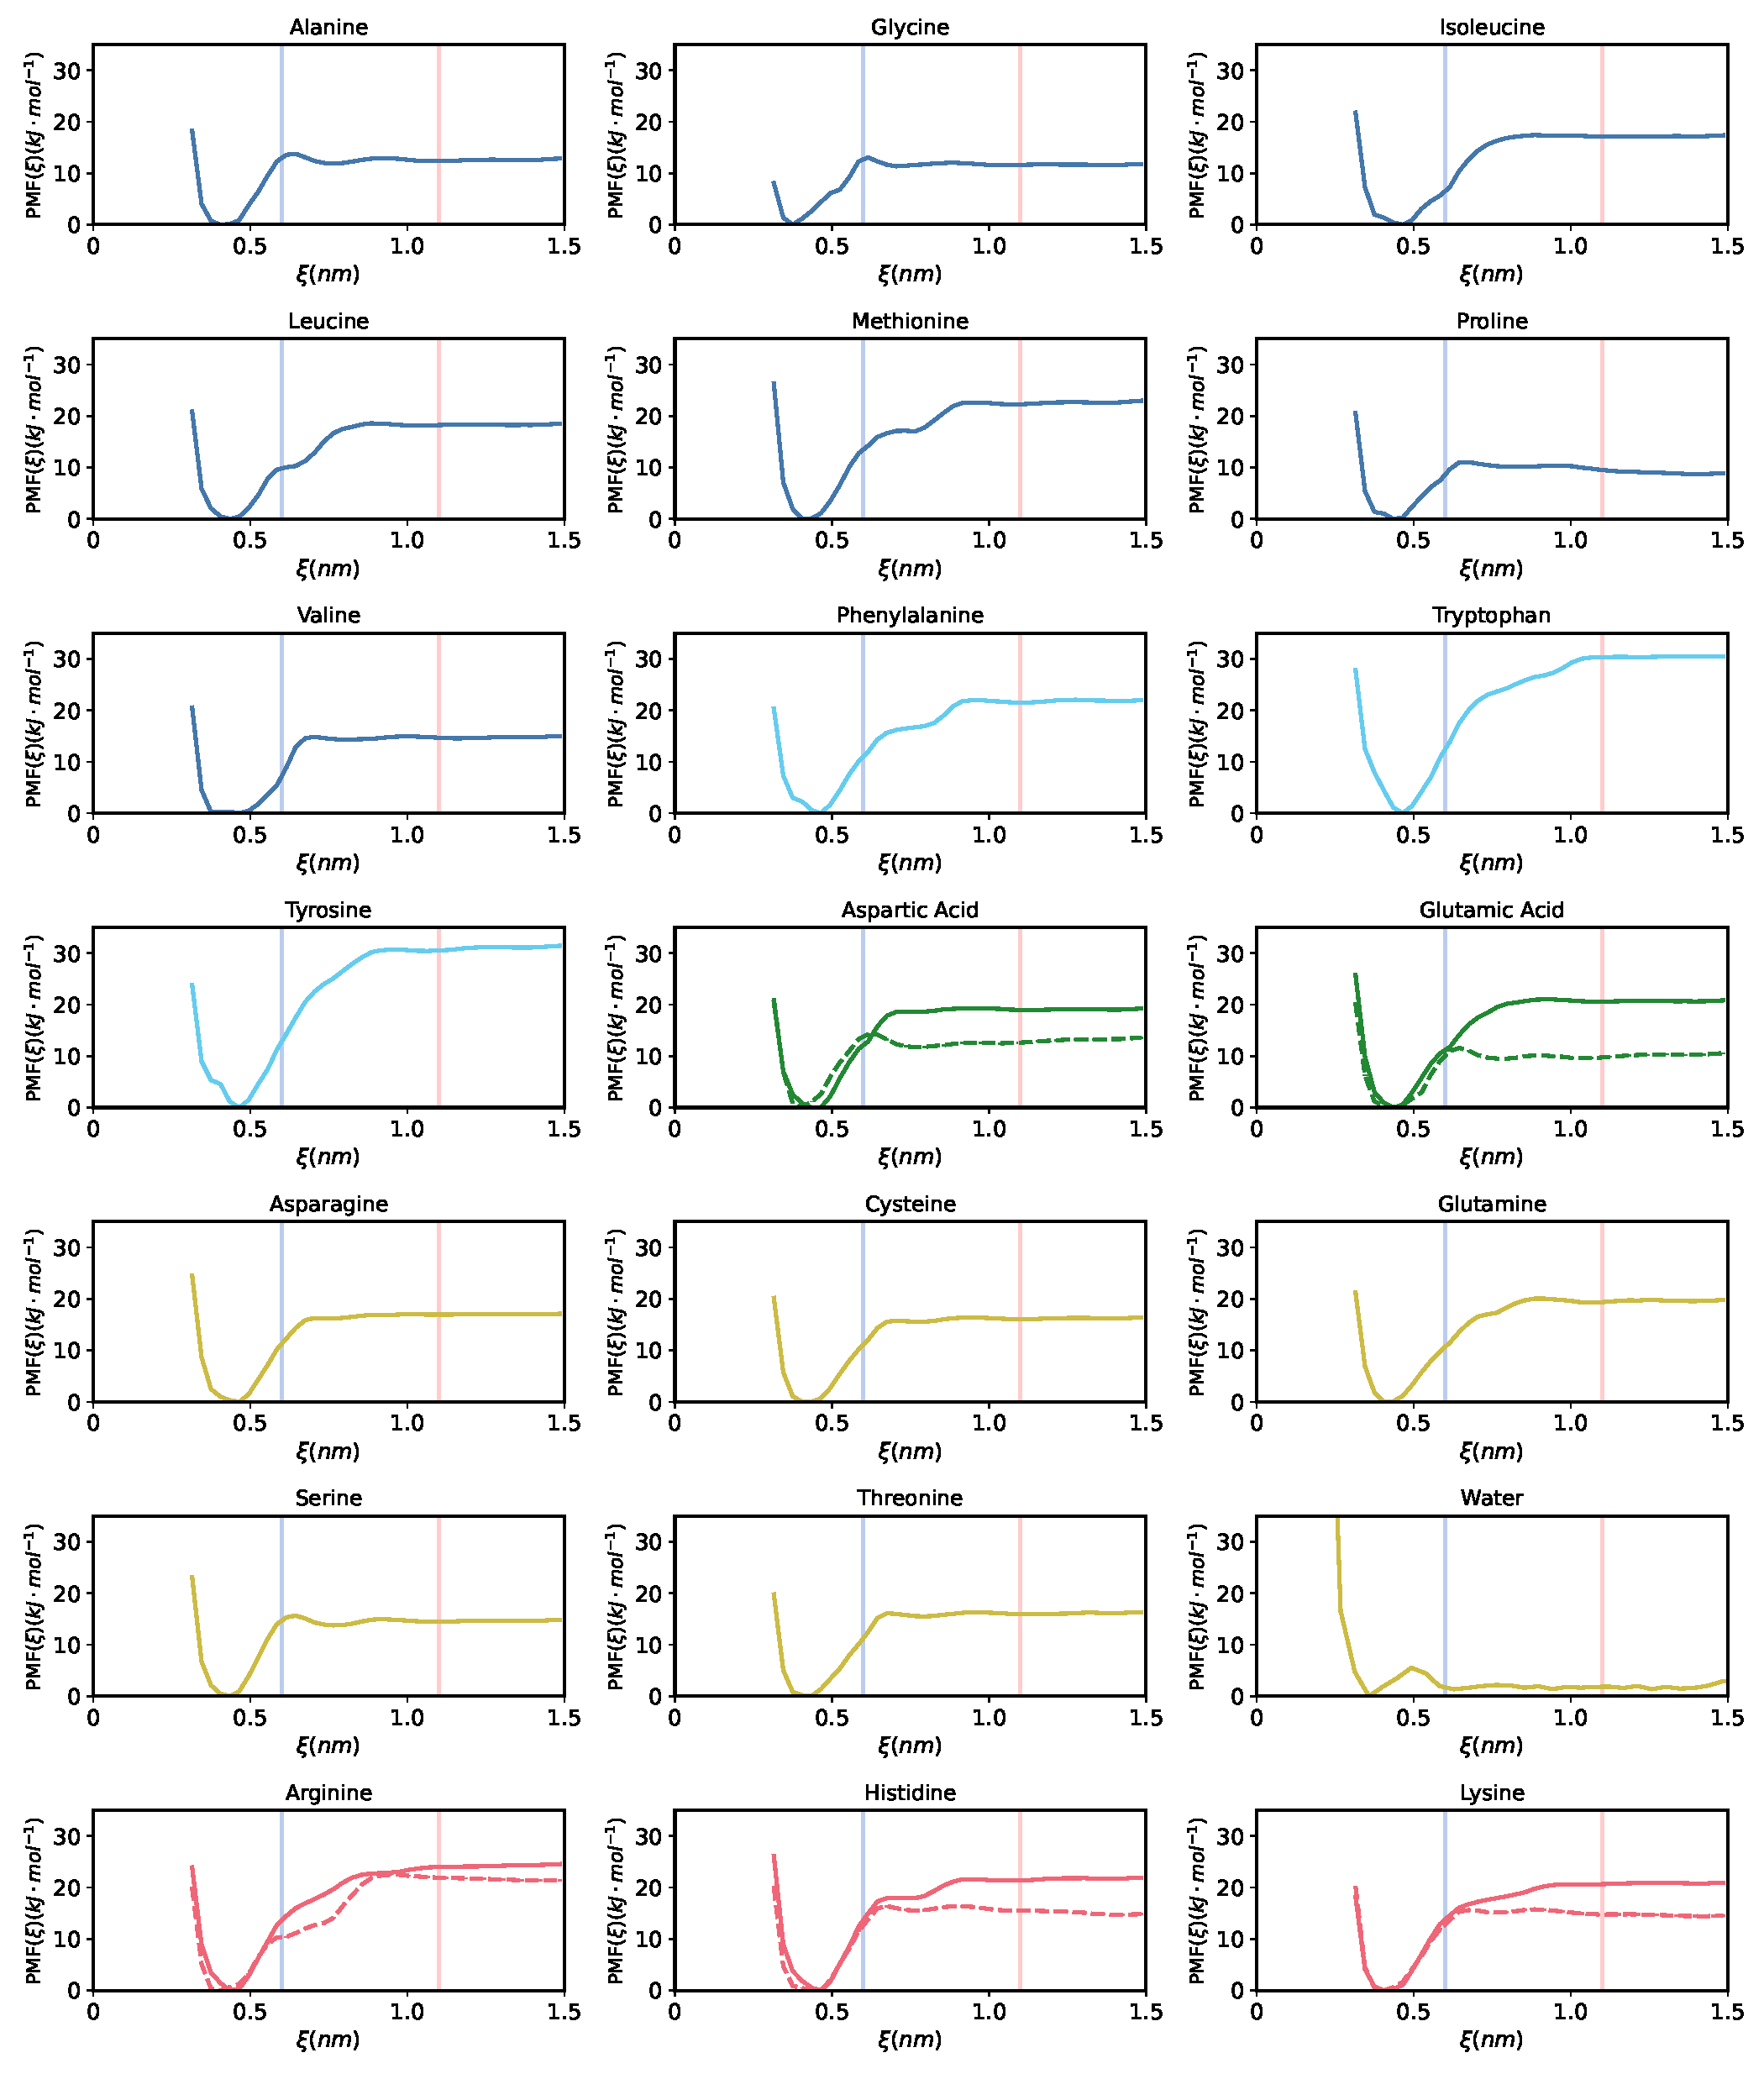
\includegraphics[width=.9\textwidth]{FigS1.pdf}
    \caption{PMFs representing the adsorption process of amino acids or water over $\xi$ (the distance between its $\alpha$-carbon and the graphene layer, along the z-axis) for pristine graphene. Amino acids are sorted by side-chain grouping: Apolar (blue), Aromatic (Cyan), Negative (Green), Polar (Yellow), and Positive (Red). Water was grouped in with polar amino acids. For the traditionally charged amino acids (Aspartic Acid, Arginine, Glutamic Acid,  Histidine, and Lysine), both the charged and neutral forms are shown in the same panel. Charged species are depicted with a dashed line. Vertical lines within each panel show the end of the "near" state (in blue) and the beginning of the "free" state (in red).}
    \label{fig:PMFs}
\end{figure}

\newpage
\subsection{Adsorption over partially oxidized graphene}
\begin{figure}[hbtp]
    \centering
    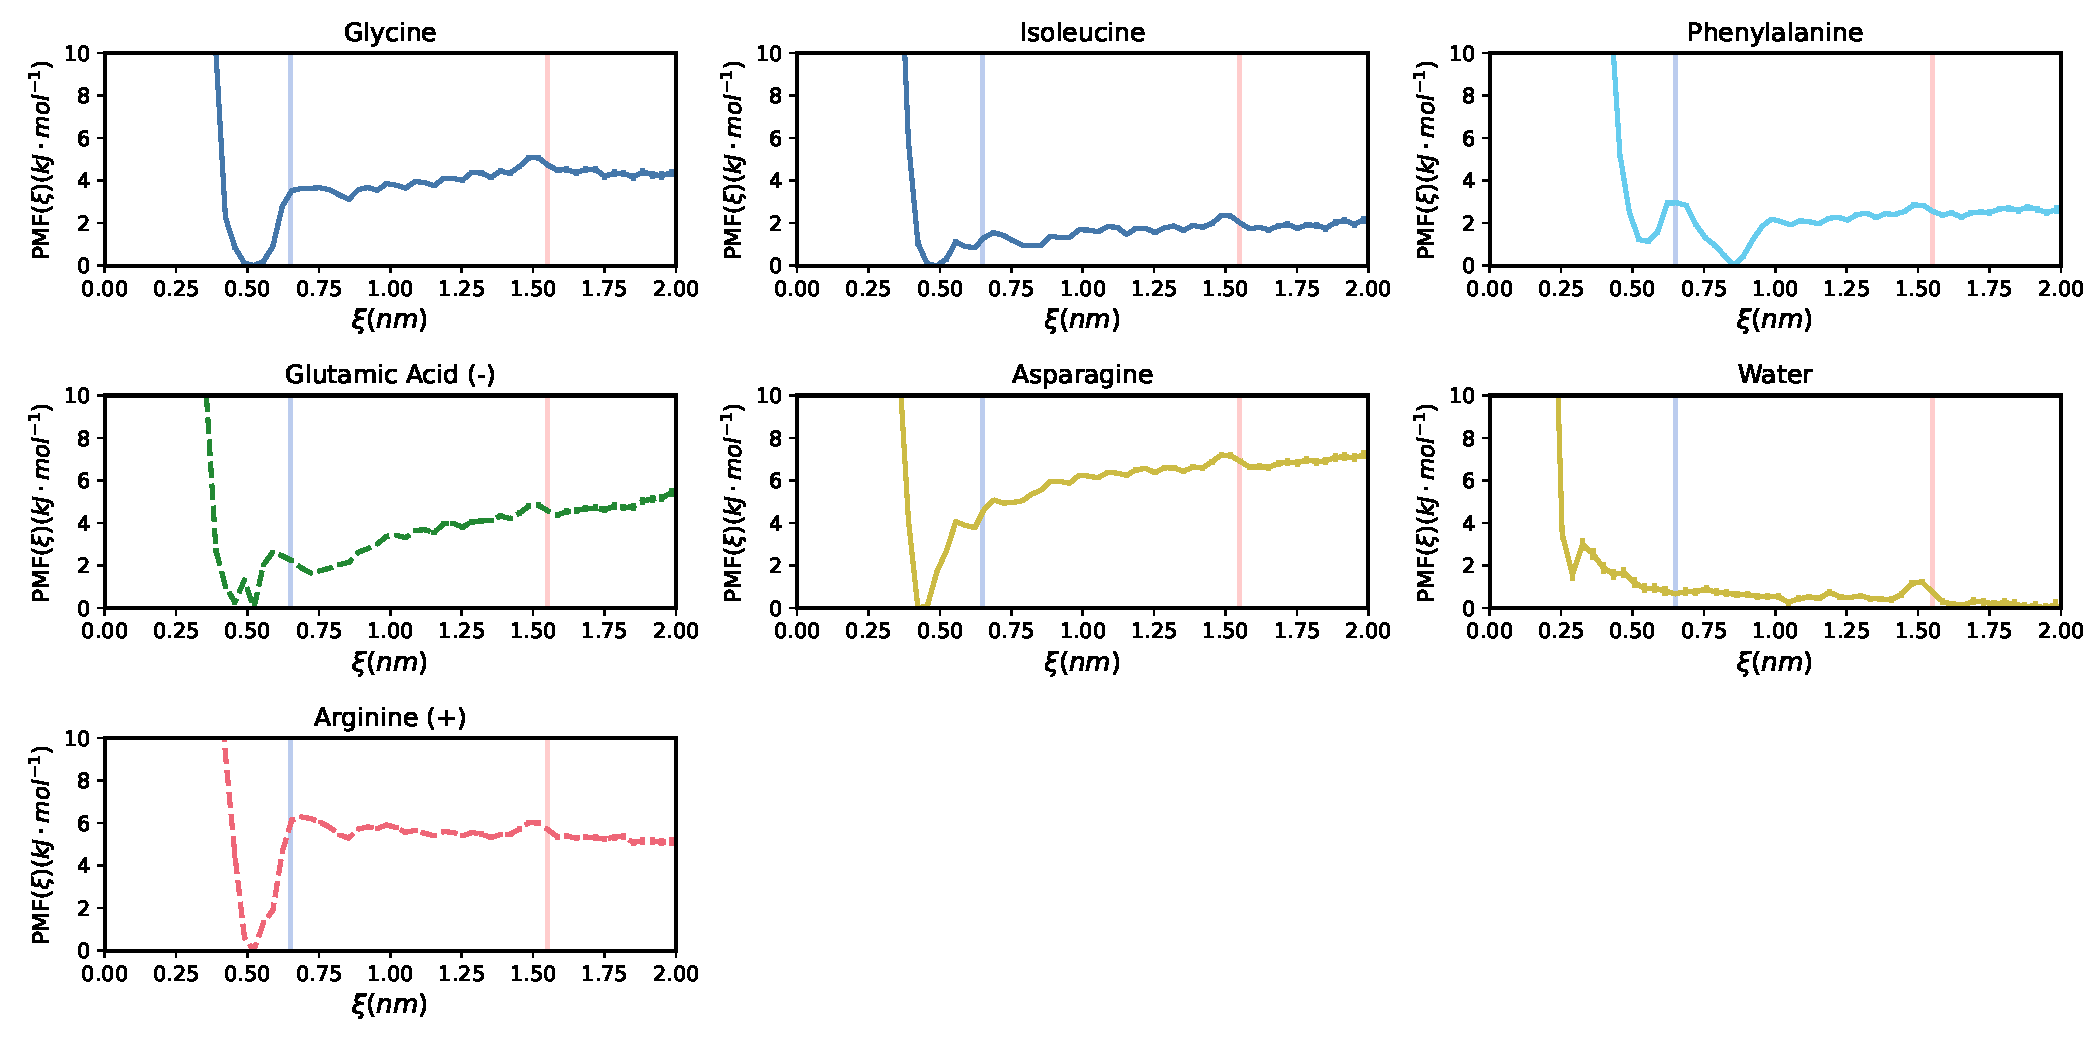
\includegraphics[width=.9\textwidth]{FigS2.pdf}
    \caption{PMFs representing the adsorption process of amino acids or water over $\xi$ for oxidized graphene. See Fig.~\ref{fig:PMFs} for details on coloring and line use.}
    \label{fig:PMFsOX}
\end{figure}

\newpage
\subsection{5--Ala adsorption}
\begin{figure}[hbtp]
    \centering
    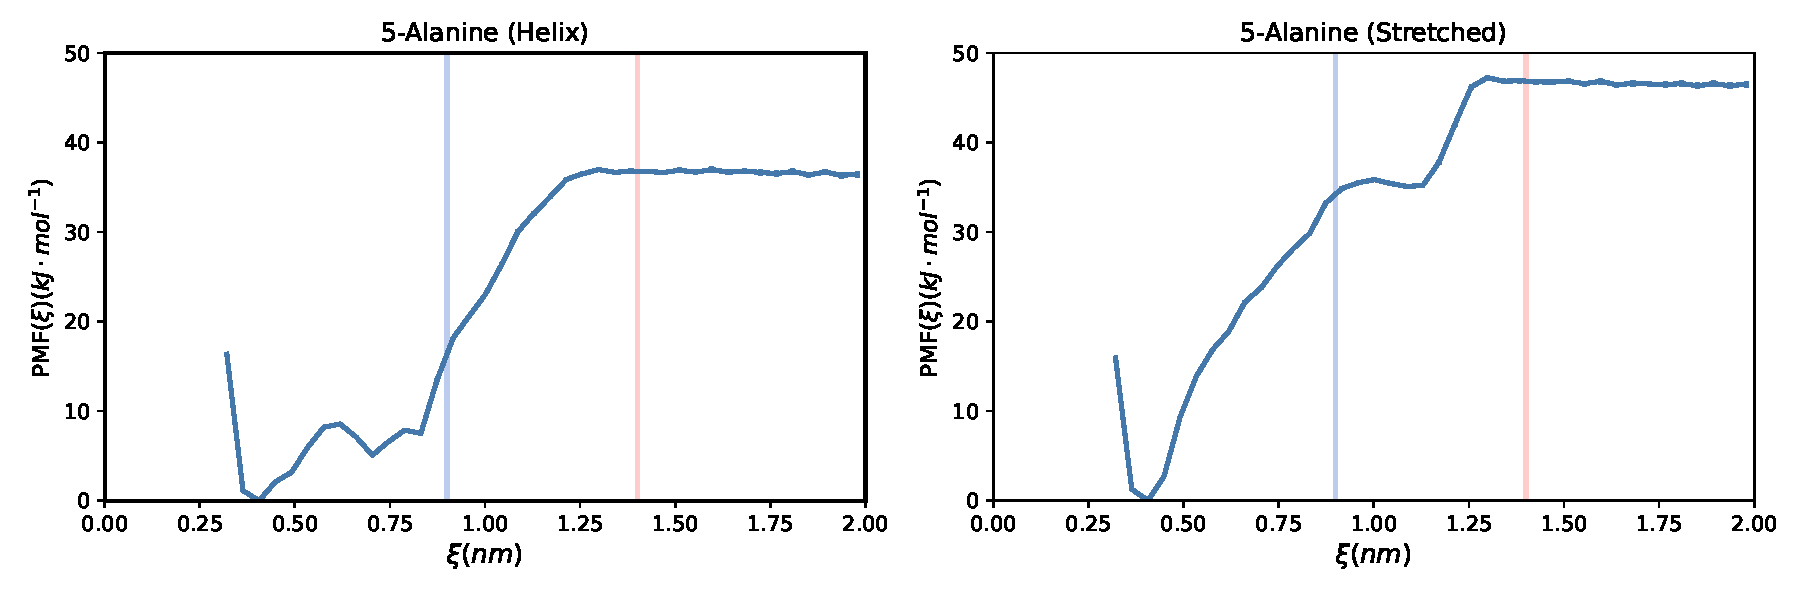
\includegraphics[width=.9\textwidth]{FigS3.pdf}
    \caption{PMFs representing the adsorption process of 5--Alanine peptides over $\xi$ above pristine graphene. See Fig.~\ref{fig:PMFs} for details on coloring and line use.}
    \label{fig:PMFs5Ala}
\end{figure}

\newpage
\section{Energy components}

\begin{table}
\centering
\caption{\label{table:PairEnergies}
Pair interaction components of the potential energy of adsorption.
}
\resizebox{\linewidth}{!}{%
\begin{tabular}{lrrrr}
\toprule
%Name              & $\Delta E^{ads}_{AA-Graph}$   & $\Delta E^{ads}_{AA-H_2O}$ & $\Delta E^{ads}_{H_2O-Graph}$ & $\Delta E^{ads}_{H_2O-H_2O}$       \\ \hline
\multirow{2}{*}{Name}  & \multicolumn{1}{r}{ $\Delta E^{ads}_{AA-Graph}$} & \multicolumn{1}{r}{$\Delta E^{ads}_{AA-H_2O}$} & \multicolumn{1}{r}{$\Delta E^{ads}_{H_2O-Graph}$} & \multicolumn{1}{r}{$\Delta E^{ads}_{H_2O-H_2O}$}  \\
\cline{2-5}            & \multicolumn{4}{c}{$[kJ \cdot mol^{-1}]$} \\ \hline
Alanine           & $-29.1 \pm 0.1$               & $  18.4 \pm 0.2$           & $21.9 \pm 0.3$                & $-22.6 \pm 1.6$                    \\
Arginine          & $-57.2 \pm 0.7$               & $  37.7 \pm 0.7$           & $36.3 \pm 1.0$                & $-58.4 \pm 3.9$                    \\
Arginine (+)      & $-60.0 \pm 0.7$               & $   7.8 \pm 1.1$           & $38.8 \pm 0.7$                & $-34.6 \pm 6.2$                    \\
Asparagine        & $-40.9 \pm 0.1$               & $  28.3 \pm 0.4$           & $24.1 \pm 0.3$                & $-33.6 \pm 1.8$                    \\
Aspartate (-) & $-34.1 \pm 0.1$               & $  31.9 \pm 0.9$           & $14.7 \pm 0.3$                & $-21.7 \pm 1.7$                    \\
Aspartic Acid     & $-41.5 \pm 0.3$               & $  21.4 \pm 0.3$           & $25.4 \pm 0.3$                & $-28.7 \pm 2.2$                    \\
Cysteine          & $-35.9 \pm 0.1$               & $  19.0 \pm 0.3$           & $24.6 \pm 0.3$                & $-22.8 \pm 1.7$                    \\
Glutamate (-) & $-37.8 \pm 0.1$               & $ 106.0 \pm 1.5$           & $17.8 \pm 0.3$                & $-53.1 \pm 1.8$                    \\
Glutamic Acid     & $-49.8 \pm 0.3$               & $  19.9 \pm 0.6$           & $29.2 \pm 1.0$                & $-29.9 \pm 3.9$                    \\
Glutamine         & $-49.1 \pm 0.1$               & $  28.9 \pm 0.3$           & $28.8 \pm 0.2$                & $-32.2 \pm 1.4$                    \\
Glycine           & $-27.4 \pm 0.0$               & $  16.1 \pm 0.2$           & $18.3 \pm 0.2$                & $-22.1 \pm 1.4$                    \\
Histidine (+)     & $-53.2 \pm 0.1$               & $  18.0 \pm 0.6$           & $35.3 \pm 0.3$                & $-38.4 \pm 1.5$                    \\
Histidine         & $-52.3 \pm 0.1$               & $  34.0 \pm 0.3$           & $31.9 \pm 0.2$                & $-36.6 \pm 1.4$                    \\
Isoleucine        & $-41.1 \pm 0.1$               & $  25.2 \pm 0.2$           & $31.9 \pm 0.3$                & $-28.9 \pm 1.5$                    \\
Leucine           & $-45.7 \pm 0.3$               & $  25.3 \pm 0.3$           & $33.0 \pm 0.3$                & $-29.7 \pm 2.0$                    \\
Lysine            & $-48.5 \pm 0.5$               & $  29.4 \pm 0.6$           & $33.9 \pm 0.7$                & $-37.2 \pm 2.5$                    \\
Lysine (+)        & $-46.4 \pm 0.1$               & $  17.2 \pm 0.9$           & $36.6 \pm 0.3$                & $-32.5 \pm 1.8$                    \\
Methionine        & $-49.9 \pm 0.7$               & $  26.0 \pm 0.7$           & $33.5 \pm 0.7$                & $-46.8 \pm 6.0$                    \\
Phenylalanine     & $-56.9 \pm 0.1$               & $  35.9 \pm 0.3$           & $38.8 \pm 0.3$                & $-42.5 \pm 1.5$                    \\
Proline           & $-35.9 \pm 0.1$               & $   6.4 \pm 0.2$           & $30.3 \pm 0.3$                & $-25.3 \pm 1.5$                    \\
Serine            & $-32.9 \pm 0.1$               & $  15.1 \pm 0.3$           & $21.0 \pm 0.3$                & $-19.4 \pm 1.6$                    \\
Threonine         & $-35.0 \pm 0.1$               & $  15.6 \pm 0.3$           & $24.6 \pm 0.3$                & $-20.2 \pm 1.5$                    \\
Tryptophan        & $-76.1 \pm 0.1$               & $  53.2 \pm 0.2$           & $47.0 \pm 0.2$                & $-50.9 \pm 1.5$                    \\
Tyrosine          & $-64.0 \pm 0.1$               & $  32.3 \pm 0.3$           & $39.6 \pm 0.3$                & $-37.1 \pm 1.6$                    \\
Valine            & $-35.9 \pm 0.1$               & $  18.7 \pm 0.3$           & $27.9 \pm 0.3$                & $-21.7 \pm 1.7$                    \\
Water             & $ -4.6 \pm 0.0$               & $   4.2 \pm 0.1$           & $ 5.6 \pm 0.5$                & $ -8.7 \pm 2.8$                    \\
\bottomrule
\end{tabular}
}
\end{table}

\begin{table}
\centering
\caption{\label{table:FreeE_minus_Energies}
Sums of pair interaction components of the energy of adsorption for the solute and its surroundings.
}
\resizebox{\linewidth}{!}{%
\begin{tabular}{lrr}
\toprule
%Name              & $\Delta E^{ads}_{H_2O-Graph, H_2O-H_2O}$  & $\Delta E^{ads}_{AA-Graph, AA-H_2O}$  \\ \hline
\multirow{2}{*}{Name}  & \multicolumn{1}{r}{$\Delta E^{ads}_{H_2O-Graph, H_2O-H_2O}$} & \multicolumn{1}{r}{$\Delta E^{ads}_{AA-Graph, AA-H_2O}$} \\
\cline{2-3}            & \multicolumn{2}{c}{$[kJ \cdot mol^{-1}]$} \\ \hline
Alanine           & $-0.7  \pm 1.6$       & $-10.7 \pm 0.2$ \\
Arginine          & $-22.1 \pm 4.0$       & $-19.5 \pm 1.0$ \\
Arginine (+)      & $4.2   \pm 6.2$       & $-52.2 \pm 1.3$ \\
Asparagine        & $-9.5  \pm 1.8$       & $-12.6 \pm 0.4$ \\
Aspartic Acid (-) & $-7.0  \pm 1.7$       & $-2.2  \pm 0.9$ \\
Aspartic Acid     & $-3.3  \pm 2.2$       & $-20.1 \pm 0.4$ \\
Cysteine          & $1.8   \pm 1.7$       & $-16.9 \pm 0.3$ \\
Glutamic Acid (-) & $-35.3 \pm 1.8$       & $68.2  \pm 1.5$ \\
Glutamic Acid     & $-0.7  \pm 4.0$       & $-29.9 \pm 0.7$ \\
Glutamine         & $-3.4  \pm 1.4$       & $-20.2 \pm 0.3$ \\
Glycine           & $-3.8  \pm 1.4$       & $-11.3 \pm 0.2$ \\
Histidine (+)     & $-3.1  \pm 1.5$       & $-35.2 \pm 0.6$ \\
Histidine         & $-4.7  \pm 1.4$       & $-18.3 \pm 0.3$ \\
Isoleucine        & $3.0   \pm 1.5$       & $-15.9 \pm 0.2$ \\
Leucine           & $3.3   \pm 2.0$       & $-20.4 \pm 0.4$ \\
Lysine            & $-3.3  \pm 2.6$       & $-19.1 \pm 0.8$ \\
Lysine (+)        & $4.1   \pm 1.8$       & $-29.2 \pm 0.9$ \\
Methionine        & $-13.3 \pm 6.0$       & $-23.9 \pm 1.0$ \\
Phenylalanine     & $-3.7  \pm 1.5$       & $-21.0 \pm 0.3$ \\
Proline           & $5.0   \pm 1.5$       & $-29.5 \pm 0.2$ \\
Serine            & $1.6   \pm 1.6$       & $-17.8 \pm 0.3$ \\
Threonine         & $4.4   \pm 1.5$       & $-19.4 \pm 0.3$ \\
Tryptophan        & $-3.9  \pm 1.5$       & $-22.9 \pm 0.2$ \\
Tyrosine          & $2.5   \pm 1.6$       & $-31.7 \pm 0.3$ \\
Valine            & $6.2   \pm 1.7$       & $-17.2 \pm 0.3$ \\
Water             & $-3.1  \pm 2.8$       & $-0.4  \pm 0.1$ \\

\bottomrule
\end{tabular}
}
\end{table}

\begin{table}
\centering
\caption{\label{table:FreeE_minus_Energies}
Difference between Free energy of adsorption and (partial sums of) the pair interaction components of the energy of adsorption.
}
\resizebox{\linewidth}{!}{%
\begin{tabular}{lrrr}
\toprule
%Name              & $\Delta A^{ads} - \Delta E^{ads}_{H_2O-Graph, H_2O-H_2O}$  & $\Delta A^{ads} - \Delta E^{ads}_{AA-Graph, AA-H_2O}$  & $(\Delta A^{ads} - \Delta E^{ads}_{AA-Graph, AA-H_2O}) * \beta$    \\ \hline
\multirow{2}{*}{Name}  & \multicolumn{1}{r}{$\Delta A^{ads} - \Delta E^{ads}_{H_2O-Graph, H_2O-H_2O}$} & \multicolumn{1}{r}{ $\Delta A^{ads} - \Delta E^{ads}_{AA-Graph, AA-H_2O}$} & \multicolumn{1}{r}{$(\Delta A^{ads} - \Delta E^{ads}_{AA-Graph, AA-H_2O}) * \beta$} \\
\cline{2-4}            & \multicolumn{3}{c}{$[kJ \cdot mol^{-1}]$} \\ \hline
Alanine           & $-8.9  \pm 1.6$  & $1.1   \pm 0.2$ & $0.4   \pm 0.1$ \\
Arginine          & $1.4   \pm 4.0$  & $-1.2  \pm 1.0$ & $-0.5  \pm 0.4$ \\
Arginine (+)      & $-22.7 \pm 6.2$  & $33.7  \pm 1.3$ & $13.6  \pm 0.5$ \\
Asparagine        & $-4.4  \pm 1.8$  & $-1.3  \pm 0.4$ & $-0.5  \pm 0.2$ \\
Aspartic Acid (-) & $-2.5  \pm 1.7$  & $-7.3  \pm 0.9$ & $-2.9  \pm 0.4$ \\
Aspartic Acid     & $-12.6 \pm 2.2$  & $4.2   \pm 0.4$ & $1.7   \pm 0.2$ \\
Cysteine          & $-15.1 \pm 1.7$  & $3.6   \pm 0.3$ & $1.5   \pm 0.1$ \\
Glutamic Acid (-) & $27.8  \pm 1.8$  & $-75.7 \pm 1.5$ & $-30.6 \pm 0.6$ \\
Glutamic Acid     & $-16.5 \pm 4.0$  & $12.7  \pm 0.7$ & $5.1   \pm 0.3$ \\
Glutamine         & $-13.0 \pm 1.4$  & $3.8   \pm 0.3$ & $1.5   \pm 0.1$ \\
Glycine           & $-4.2  \pm 1.4$  & $3.3   \pm 0.2$ & $1.3   \pm 0.1$ \\
Histidine (+)     & $-9.2  \pm 1.5$  & $22.9  \pm 0.6$ & $9.2   \pm 0.2$ \\
Histidine         & $-13.5 \pm 1.4$  & $0.1   \pm 0.3$ & $0.0   \pm 0.1$ \\
Isoleucine        & $-17.3 \pm 1.5$  & $1.6   \pm 0.2$ & $0.6   \pm 0.1$ \\
Leucine           & $-18.6 \pm 2.0$  & $5.1   \pm 0.4$ & $2.1   \pm 0.2$ \\
Lysine            & $-14.4 \pm 2.6$  & $1.4   \pm 0.8$ & $0.6   \pm 0.3$ \\
Lysine (+)        & $-15.5 \pm 1.8$  & $17.8  \pm 0.9$ & $7.2   \pm 0.4$ \\
Methionine        & $-6.1  \pm 6.0$  & $4.5   \pm 1.0$ & $1.8   \pm 0.4$ \\
Phenylalanine     & $-14.7 \pm 1.5$  & $2.6   \pm 0.3$ & $1.0   \pm 0.1$ \\
Proline           & $-11.0 \pm 1.5$  & $23.5  \pm 0.2$ & $9.5   \pm 0.1$ \\
Serine            & $-12.8 \pm 1.6$  & $6.6   \pm 0.3$ & $2.7   \pm 0.1$ \\
Threonine         & $-17.4 \pm 1.5$  & $6.4   \pm 0.3$ & $2.6   \pm 0.1$ \\
Tryptophan        & $-22.3 \pm 1.5$  & $-3.3  \pm 0.2$ & $-1.3  \pm 0.1$ \\
Tyrosine          & $-30.0 \pm 1.6$  & $4.2   \pm 0.3$ & $1.7   \pm 0.1$ \\
Valine            & $-18.8 \pm 1.7$  & $4.6   \pm 0.3$ & $1.9   \pm 0.1$ \\
Water             & $6.4   \pm 2.8$  & $3.7   \pm 0.1$ & $1.5   \pm 0.1$ \\
\bottomrule
\end{tabular}
}
\end{table}



\begin{figure}[hbtp]
    \centering
    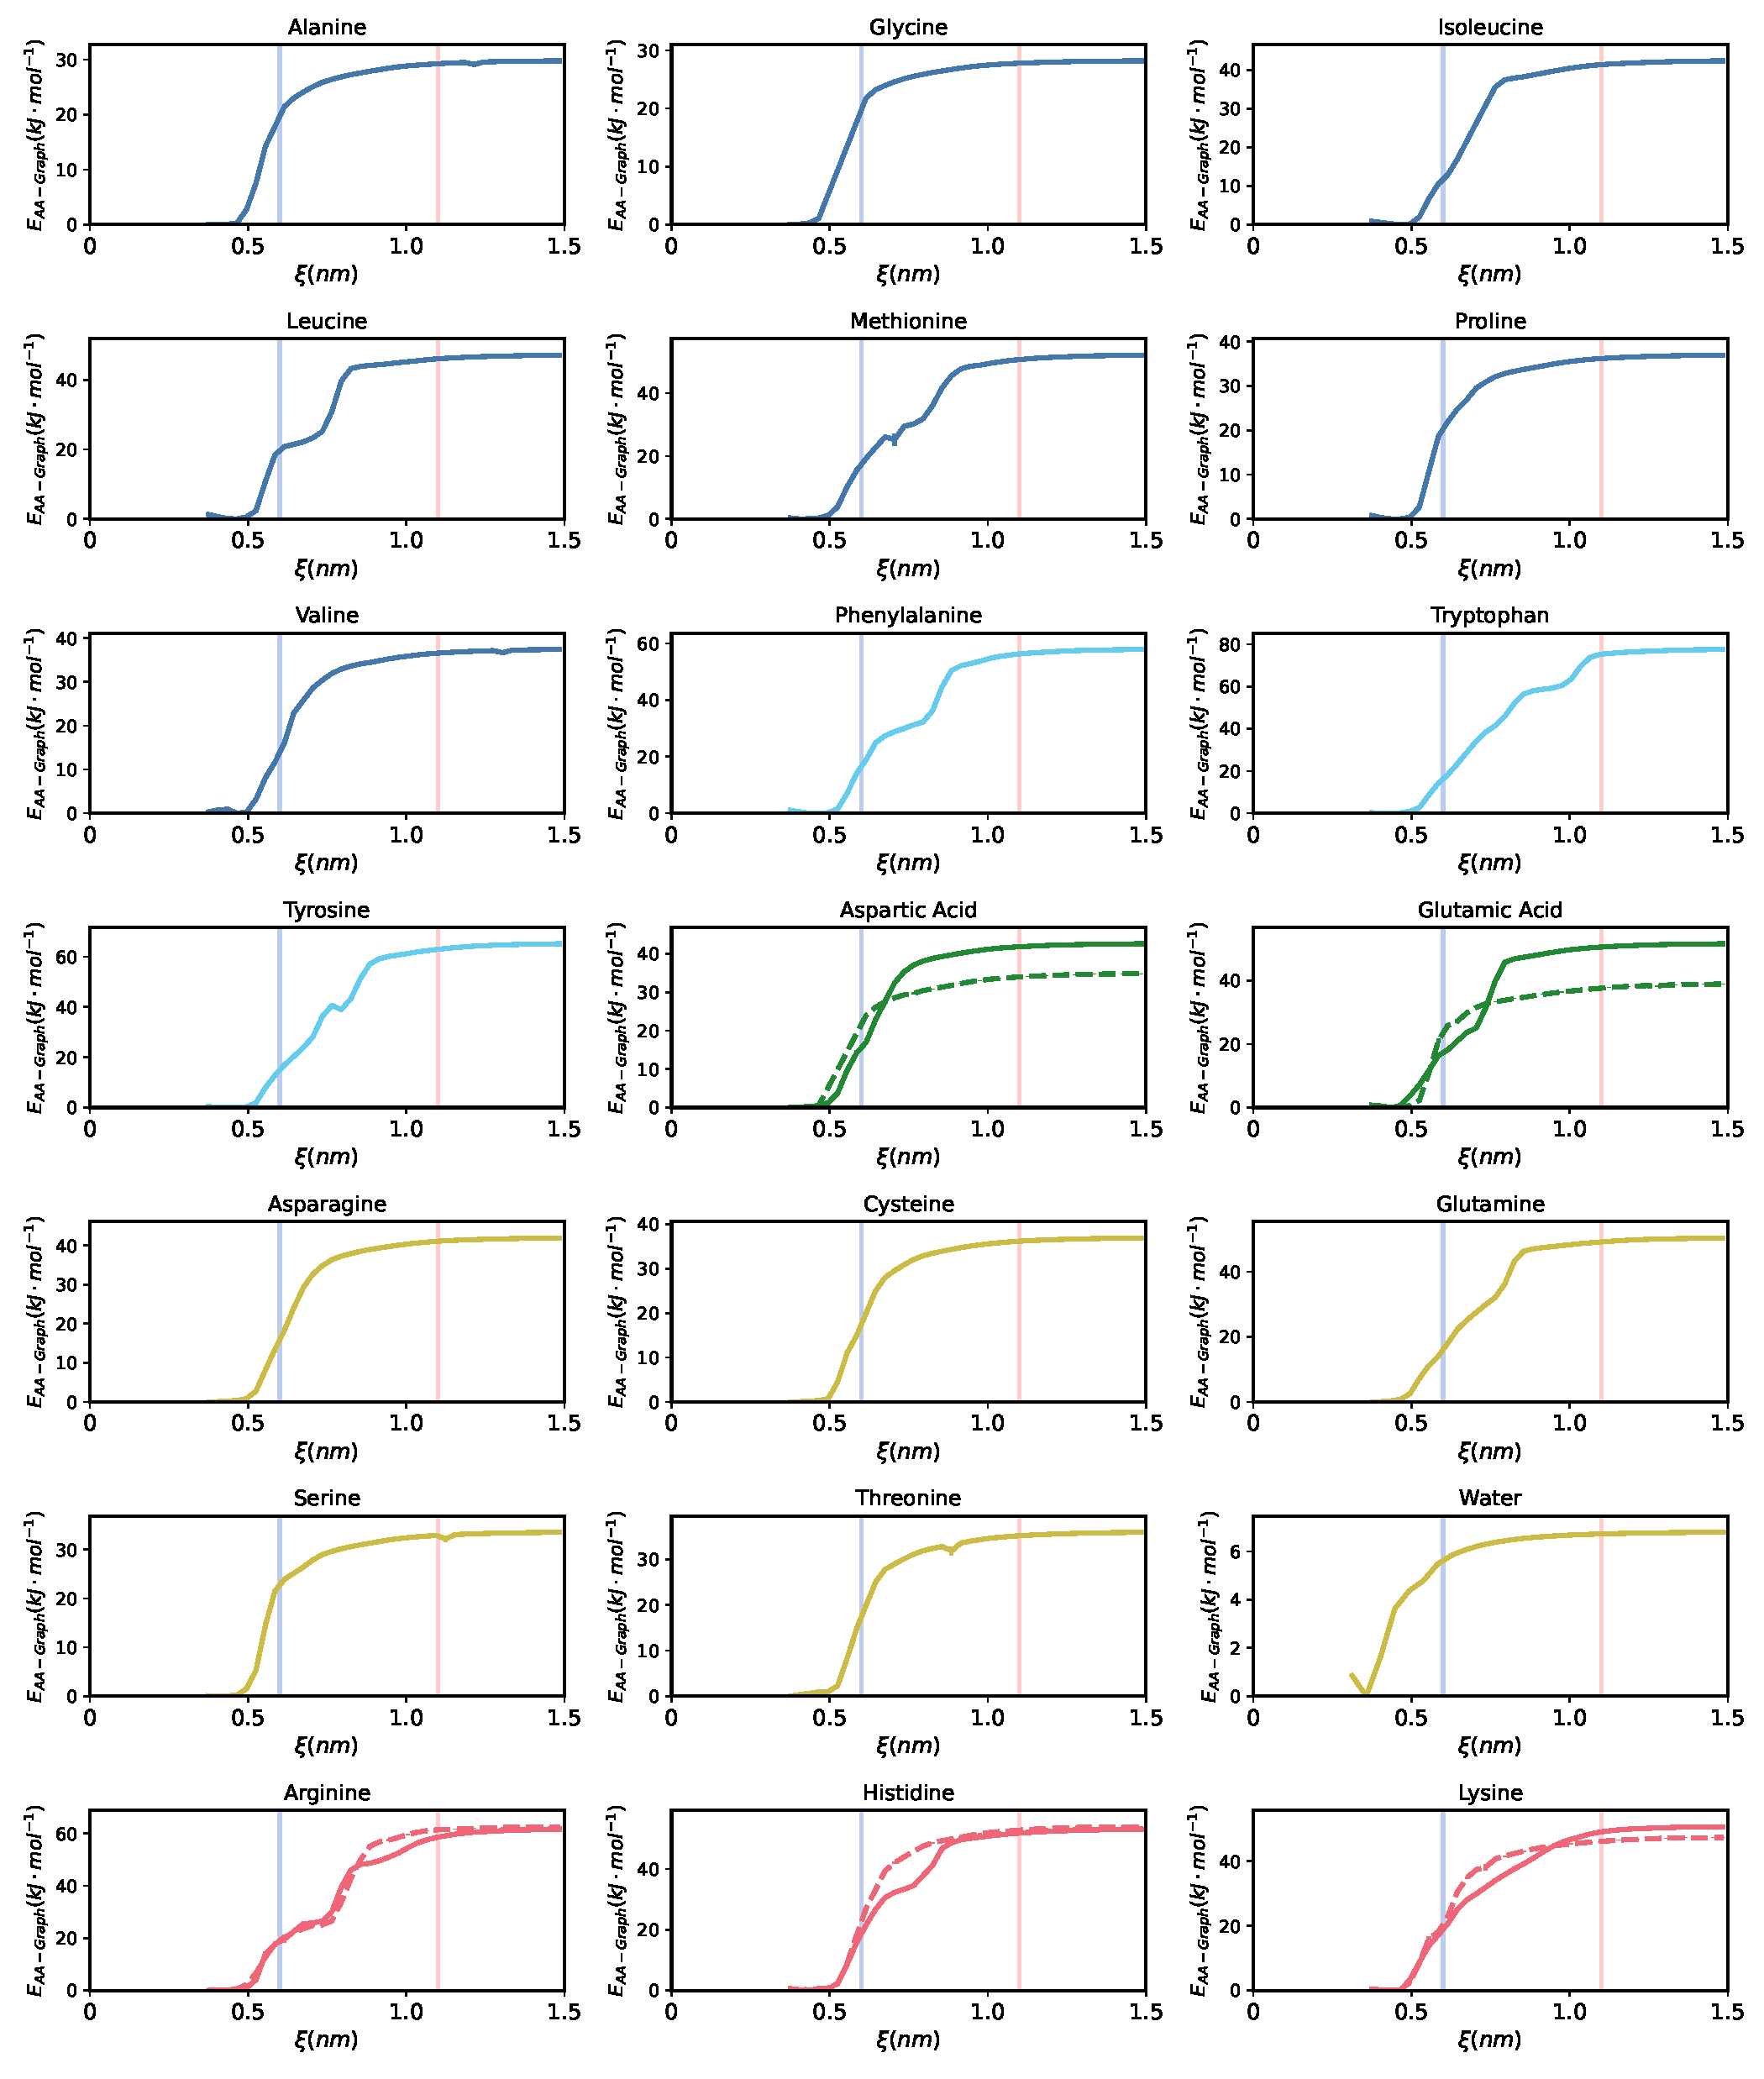
\includegraphics[width=\textwidth]{FigS4.pdf}
    \caption{Unbiased Amino-acid--Graphene interaction energy of the adsorption process of amino acids (or water) as a function of $\xi$ (the distance between its $\alpha$-carbon and the graphene layer, along the z-axis). Amino acids are sorted by side-chain grouping: Apolar (blue), Aromatic (Cyan), Negative (Green), Polar (Yellow), and Positive (Red). Water was grouped in with polar amino acids. For the traditionally charged amino acids (Aspartic Acid, Arginine, Glutamic Acid,  Histidine, and Lysine), both the charged and neutral forms are shown in the same panel. Charged species are depicted in a dashed line. Vertical lines are used to show the end of the "near" state (in blue) and the beginning of the "free" state (in red).}
    \label{fig:EnergyAA-G}
\end{figure}

\begin{figure}[hbtp]
    \centering
    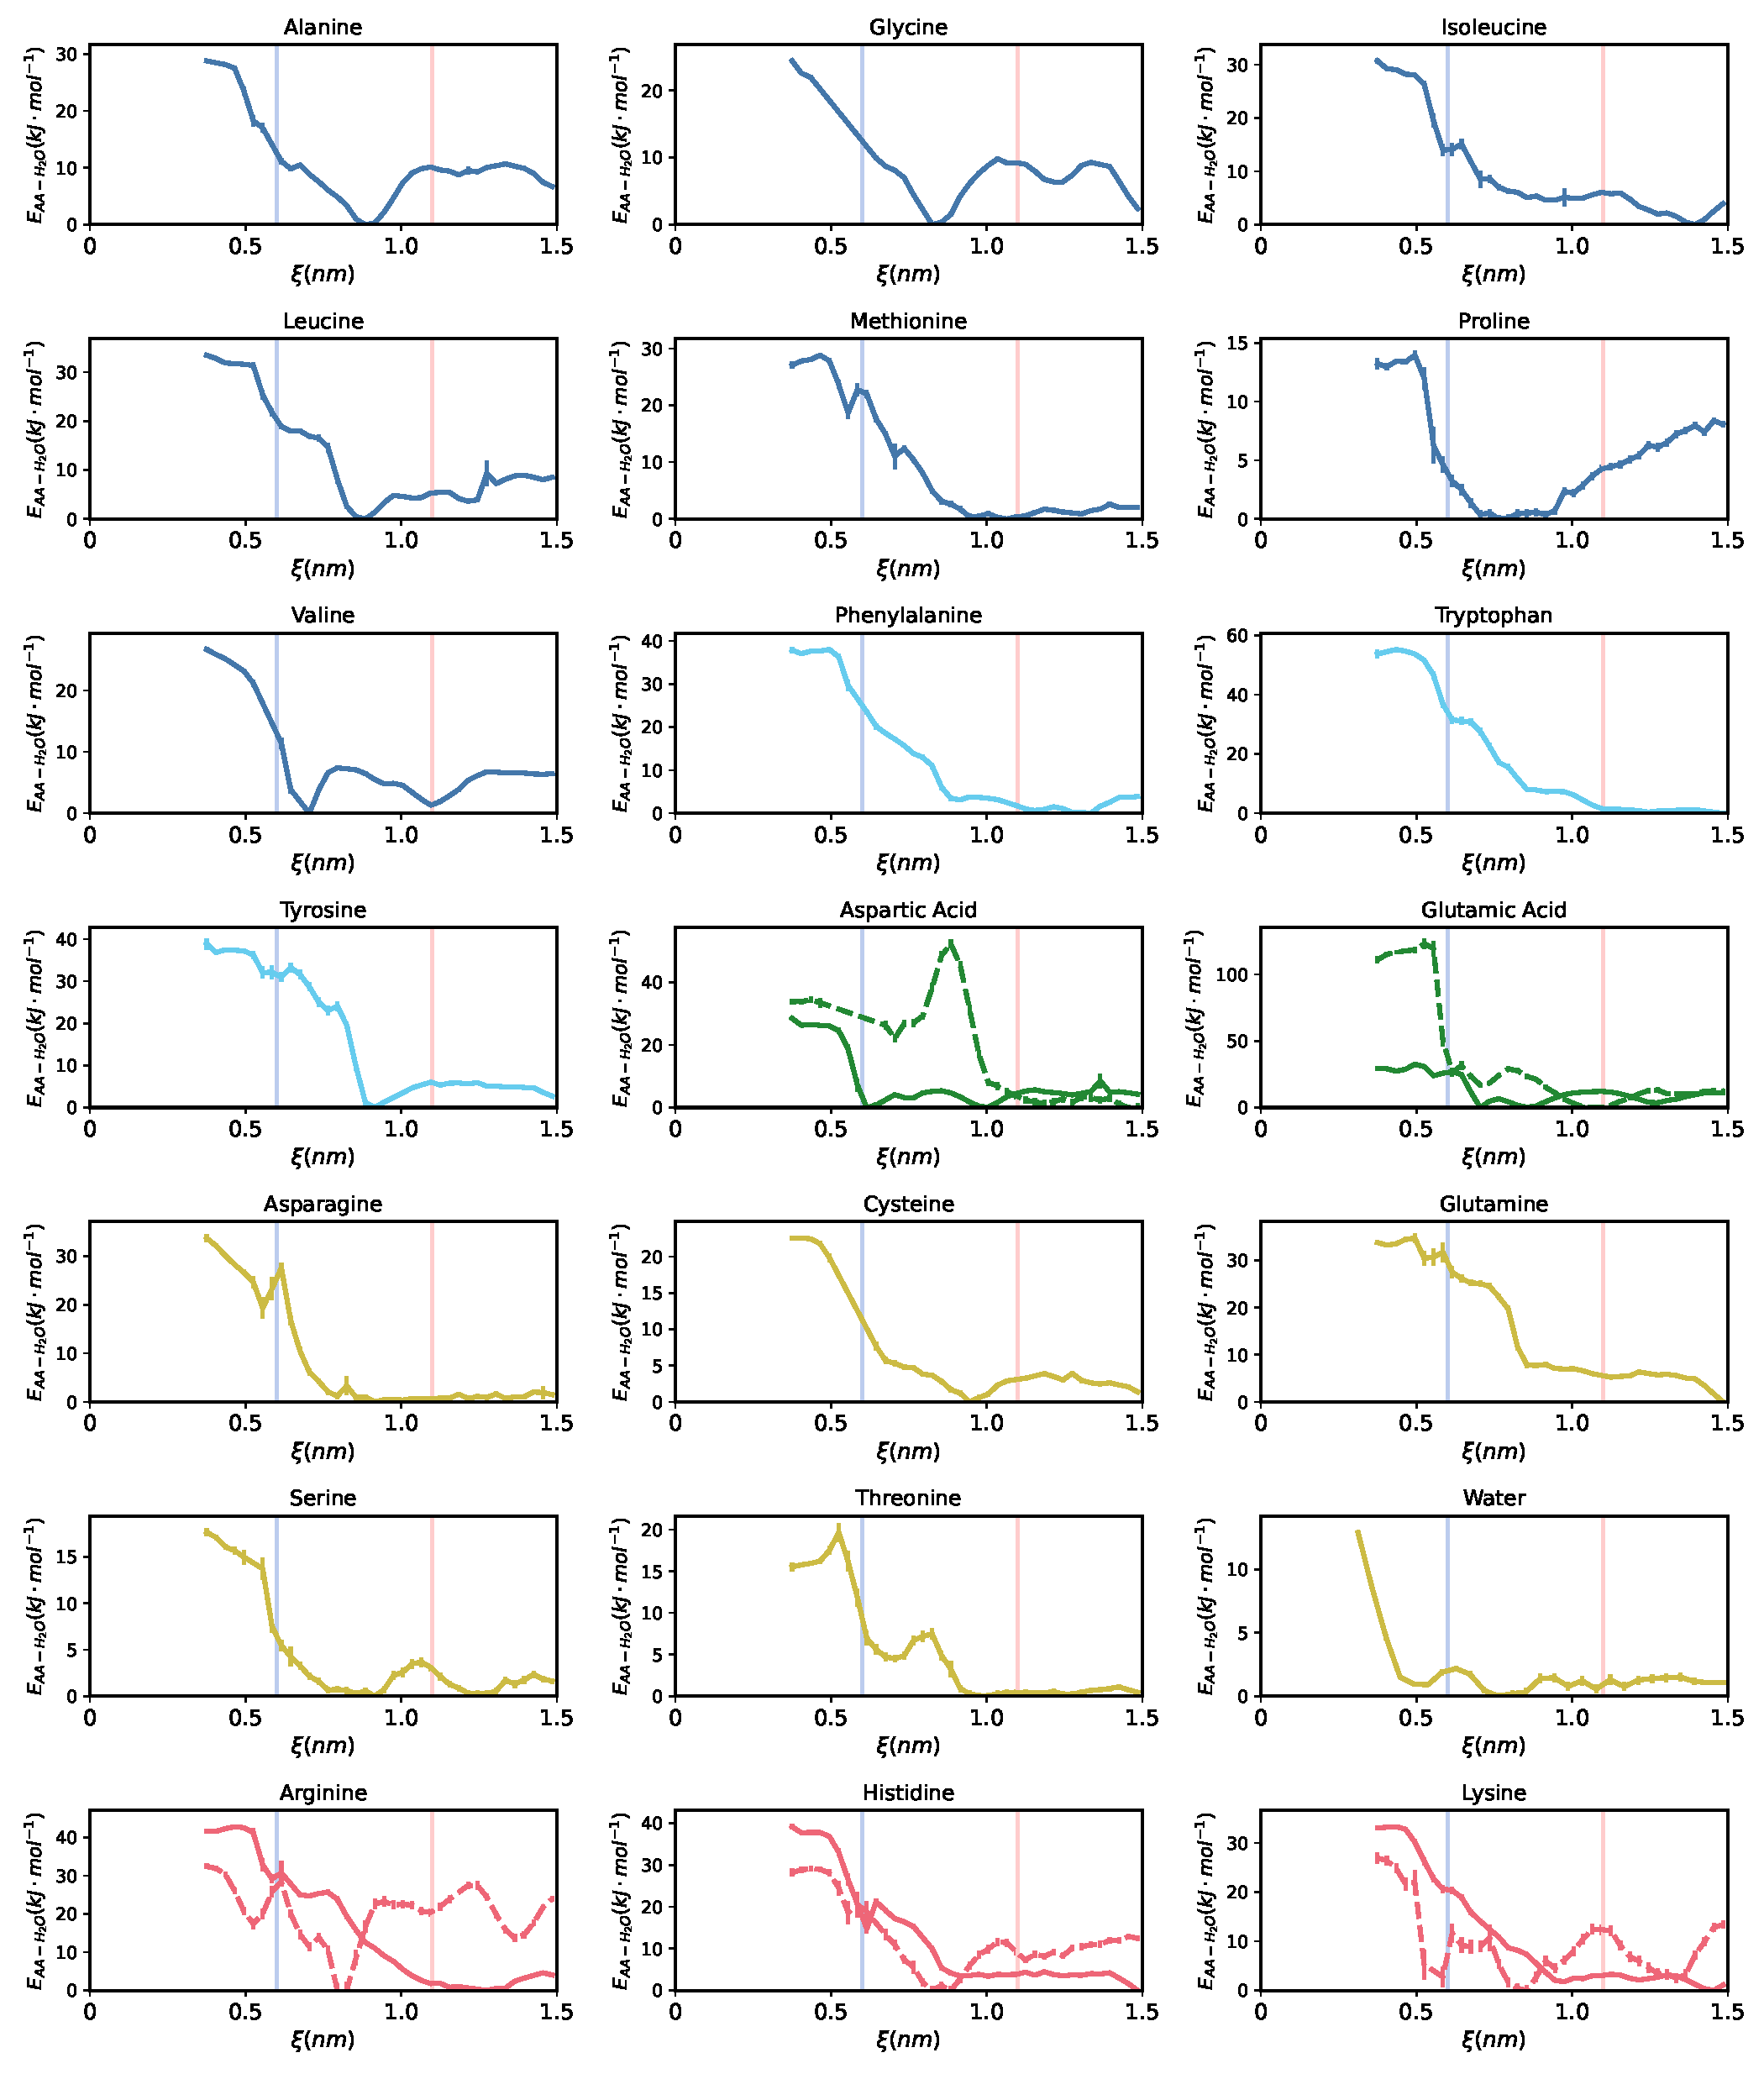
\includegraphics[width=\textwidth]{FigS5.pdf}
    \caption{Unbiased Amino-acid--Water interaction energy of the adsorption process of amino acids (or water) as a function of $\xi$ (the distance between its $\alpha$-carbon and the graphene layer, along the z-axis). Amino acids are sorted by side-chain grouping: Apolar (blue), Aromatic (Cyan), Negative (Green), Polar (Yellow), and Positive (Red). Water was grouped in with polar amino acids. For the traditionally charged amino acids (Aspartic Acid, Arginine, Glutamic Acid,  Histidine, and Lysine), both the charged and neutral forms are shown in the same panel. Charged species are depicted in a dashed line. Vertical lines are used to show the end of the "near" state (in blue) and the beginning of the "free" state (in red).}
    \label{fig:EnergyAA-W}
\end{figure}

\begin{figure}[hbtp]
    \centering
    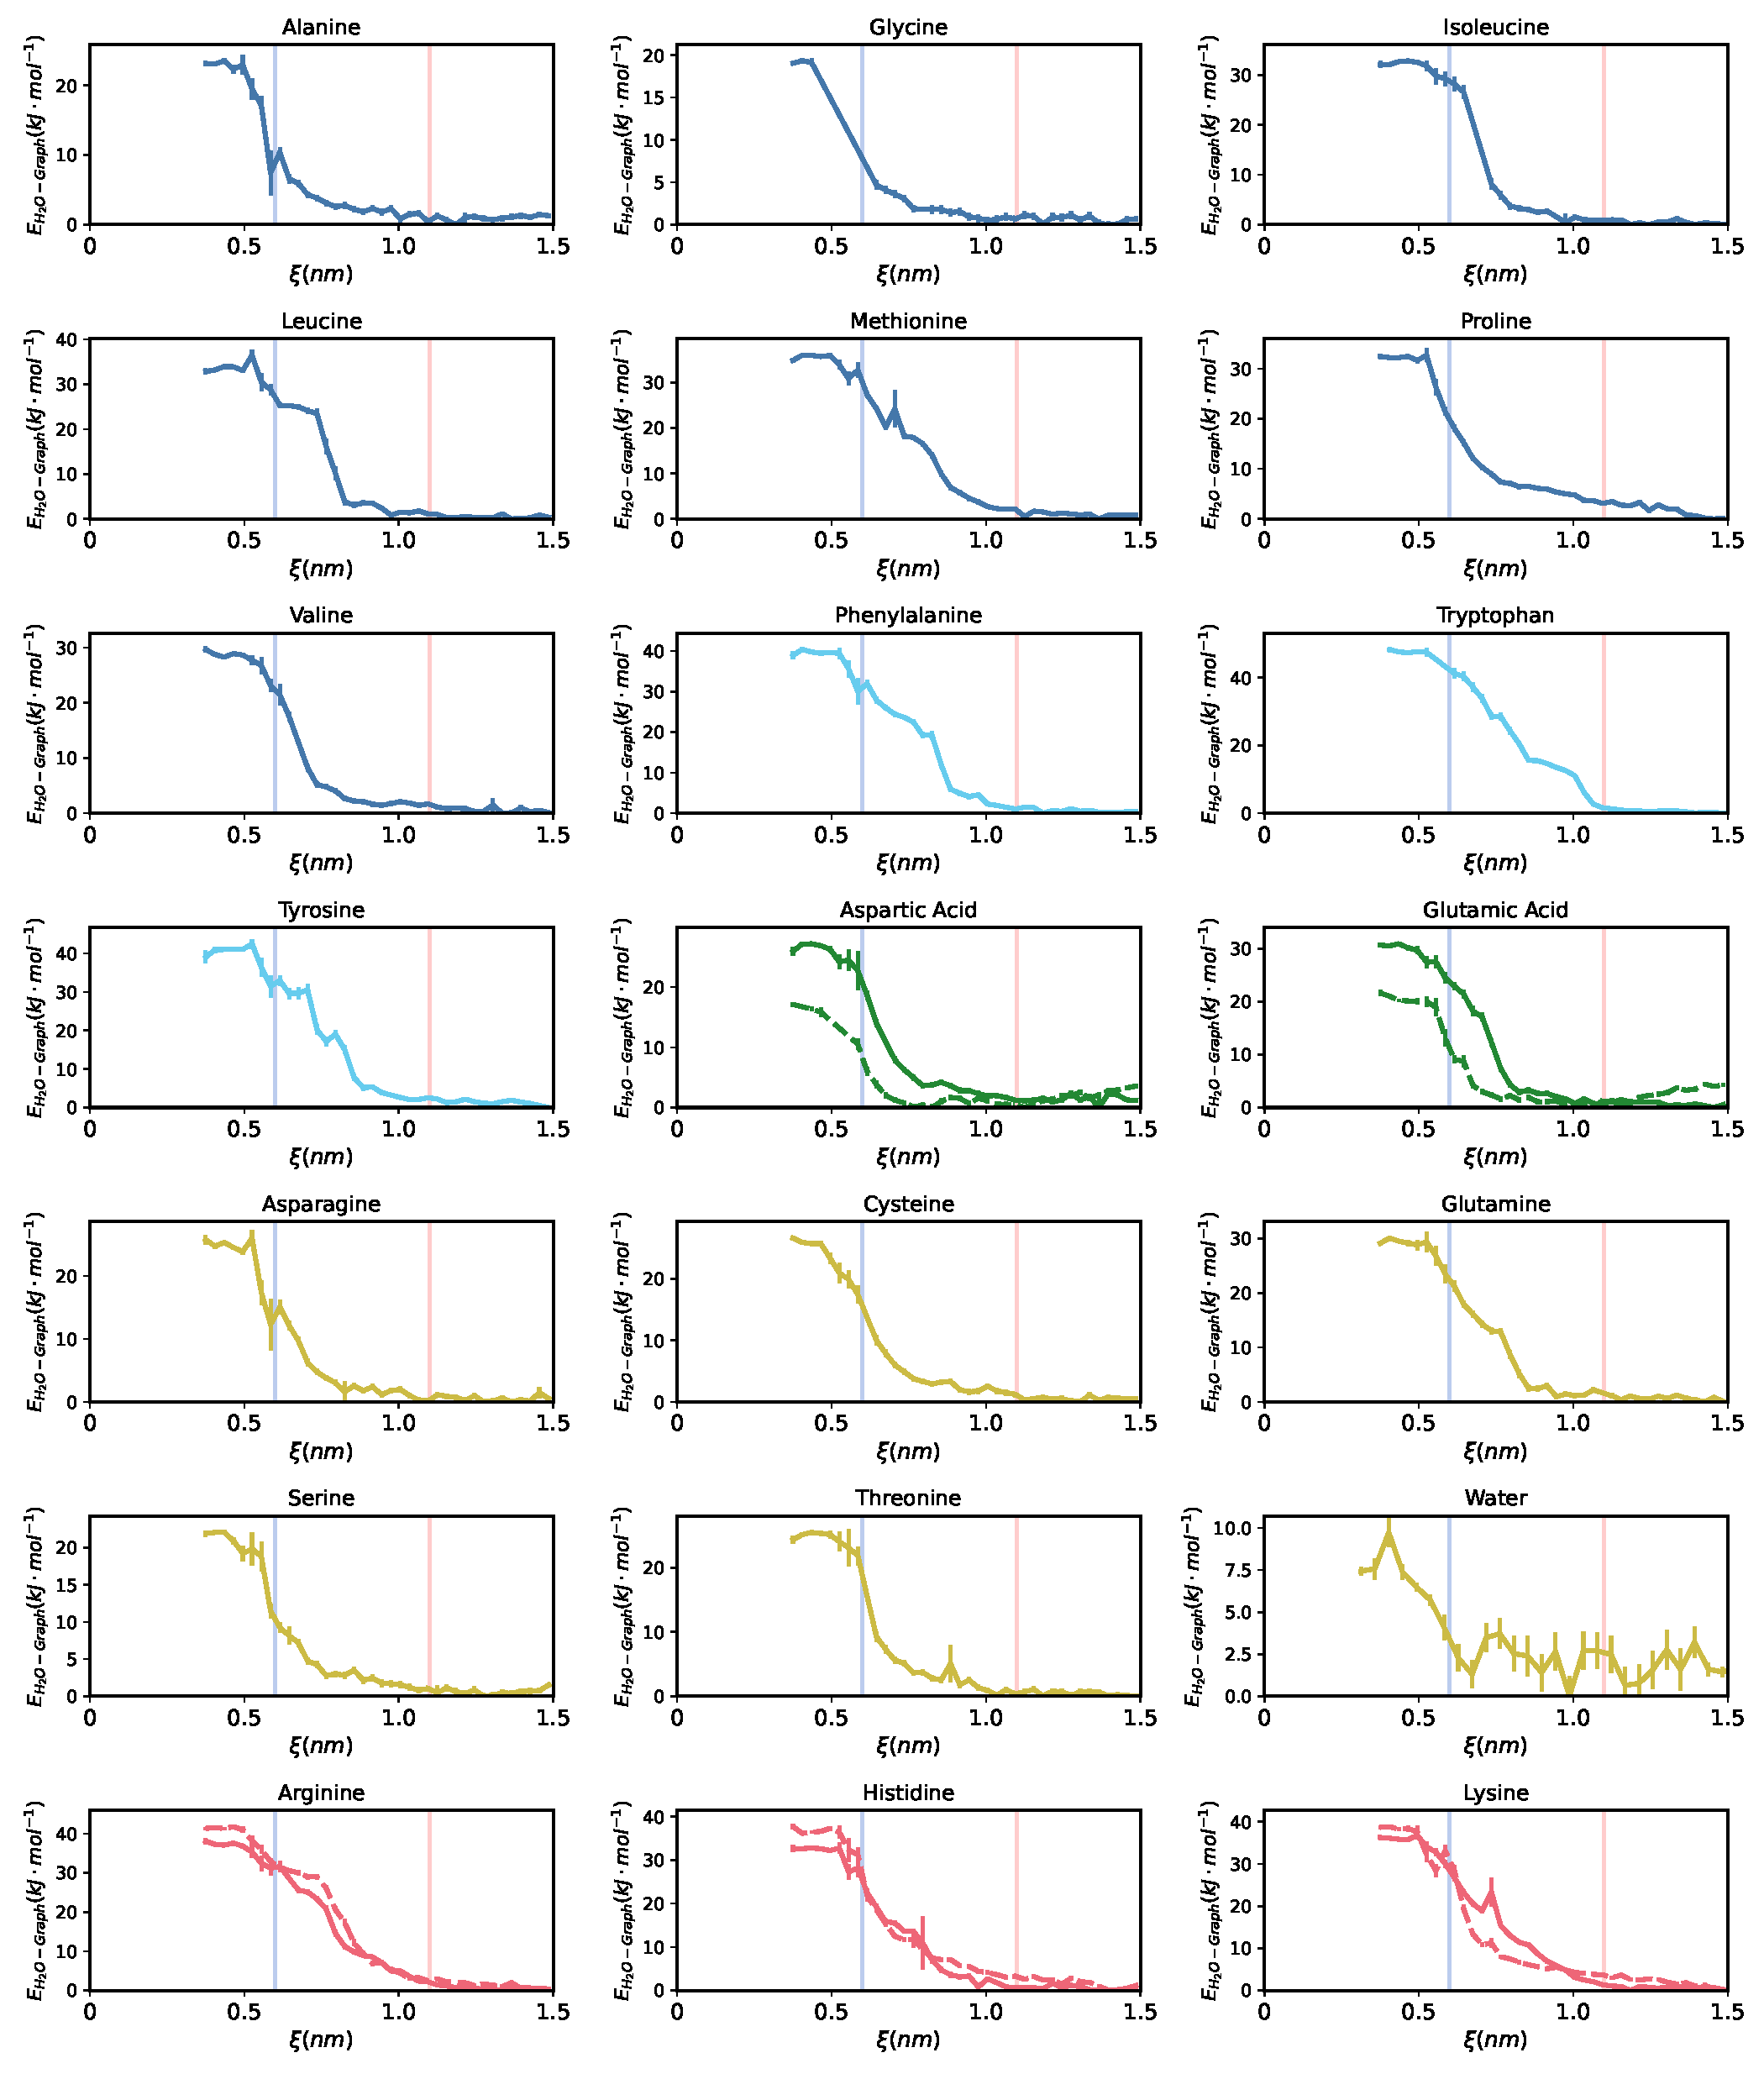
\includegraphics[width=\textwidth]{FigS6.pdf}
    \caption{Unbiased Water--Graphene interaction energy of the adsorption process of amino acids (or water) as a function of $\xi$ (the distance between its $\alpha$-carbon and the graphene layer, along the z-axis). Amino acids are sorted by side-chain grouping: Apolar (blue), Aromatic (Cyan), Negative (Green), Polar (Yellow), and Positive (Red). Water was grouped in with polar amino acids. For the traditionally charged amino acids (Aspartic Acid, Arginine, Glutamic Acid,  Histidine, and Lysine), both the charged and neutral forms are shown in the same panel. Charged species are depicted in a dashed line. Vertical lines are used to show the end of the "near" state (in blue) and the beginning of the "free" state (in red).}
    \label{fig:EnergyW-G}
\end{figure}

\begin{figure}[hbtp]
    \centering
    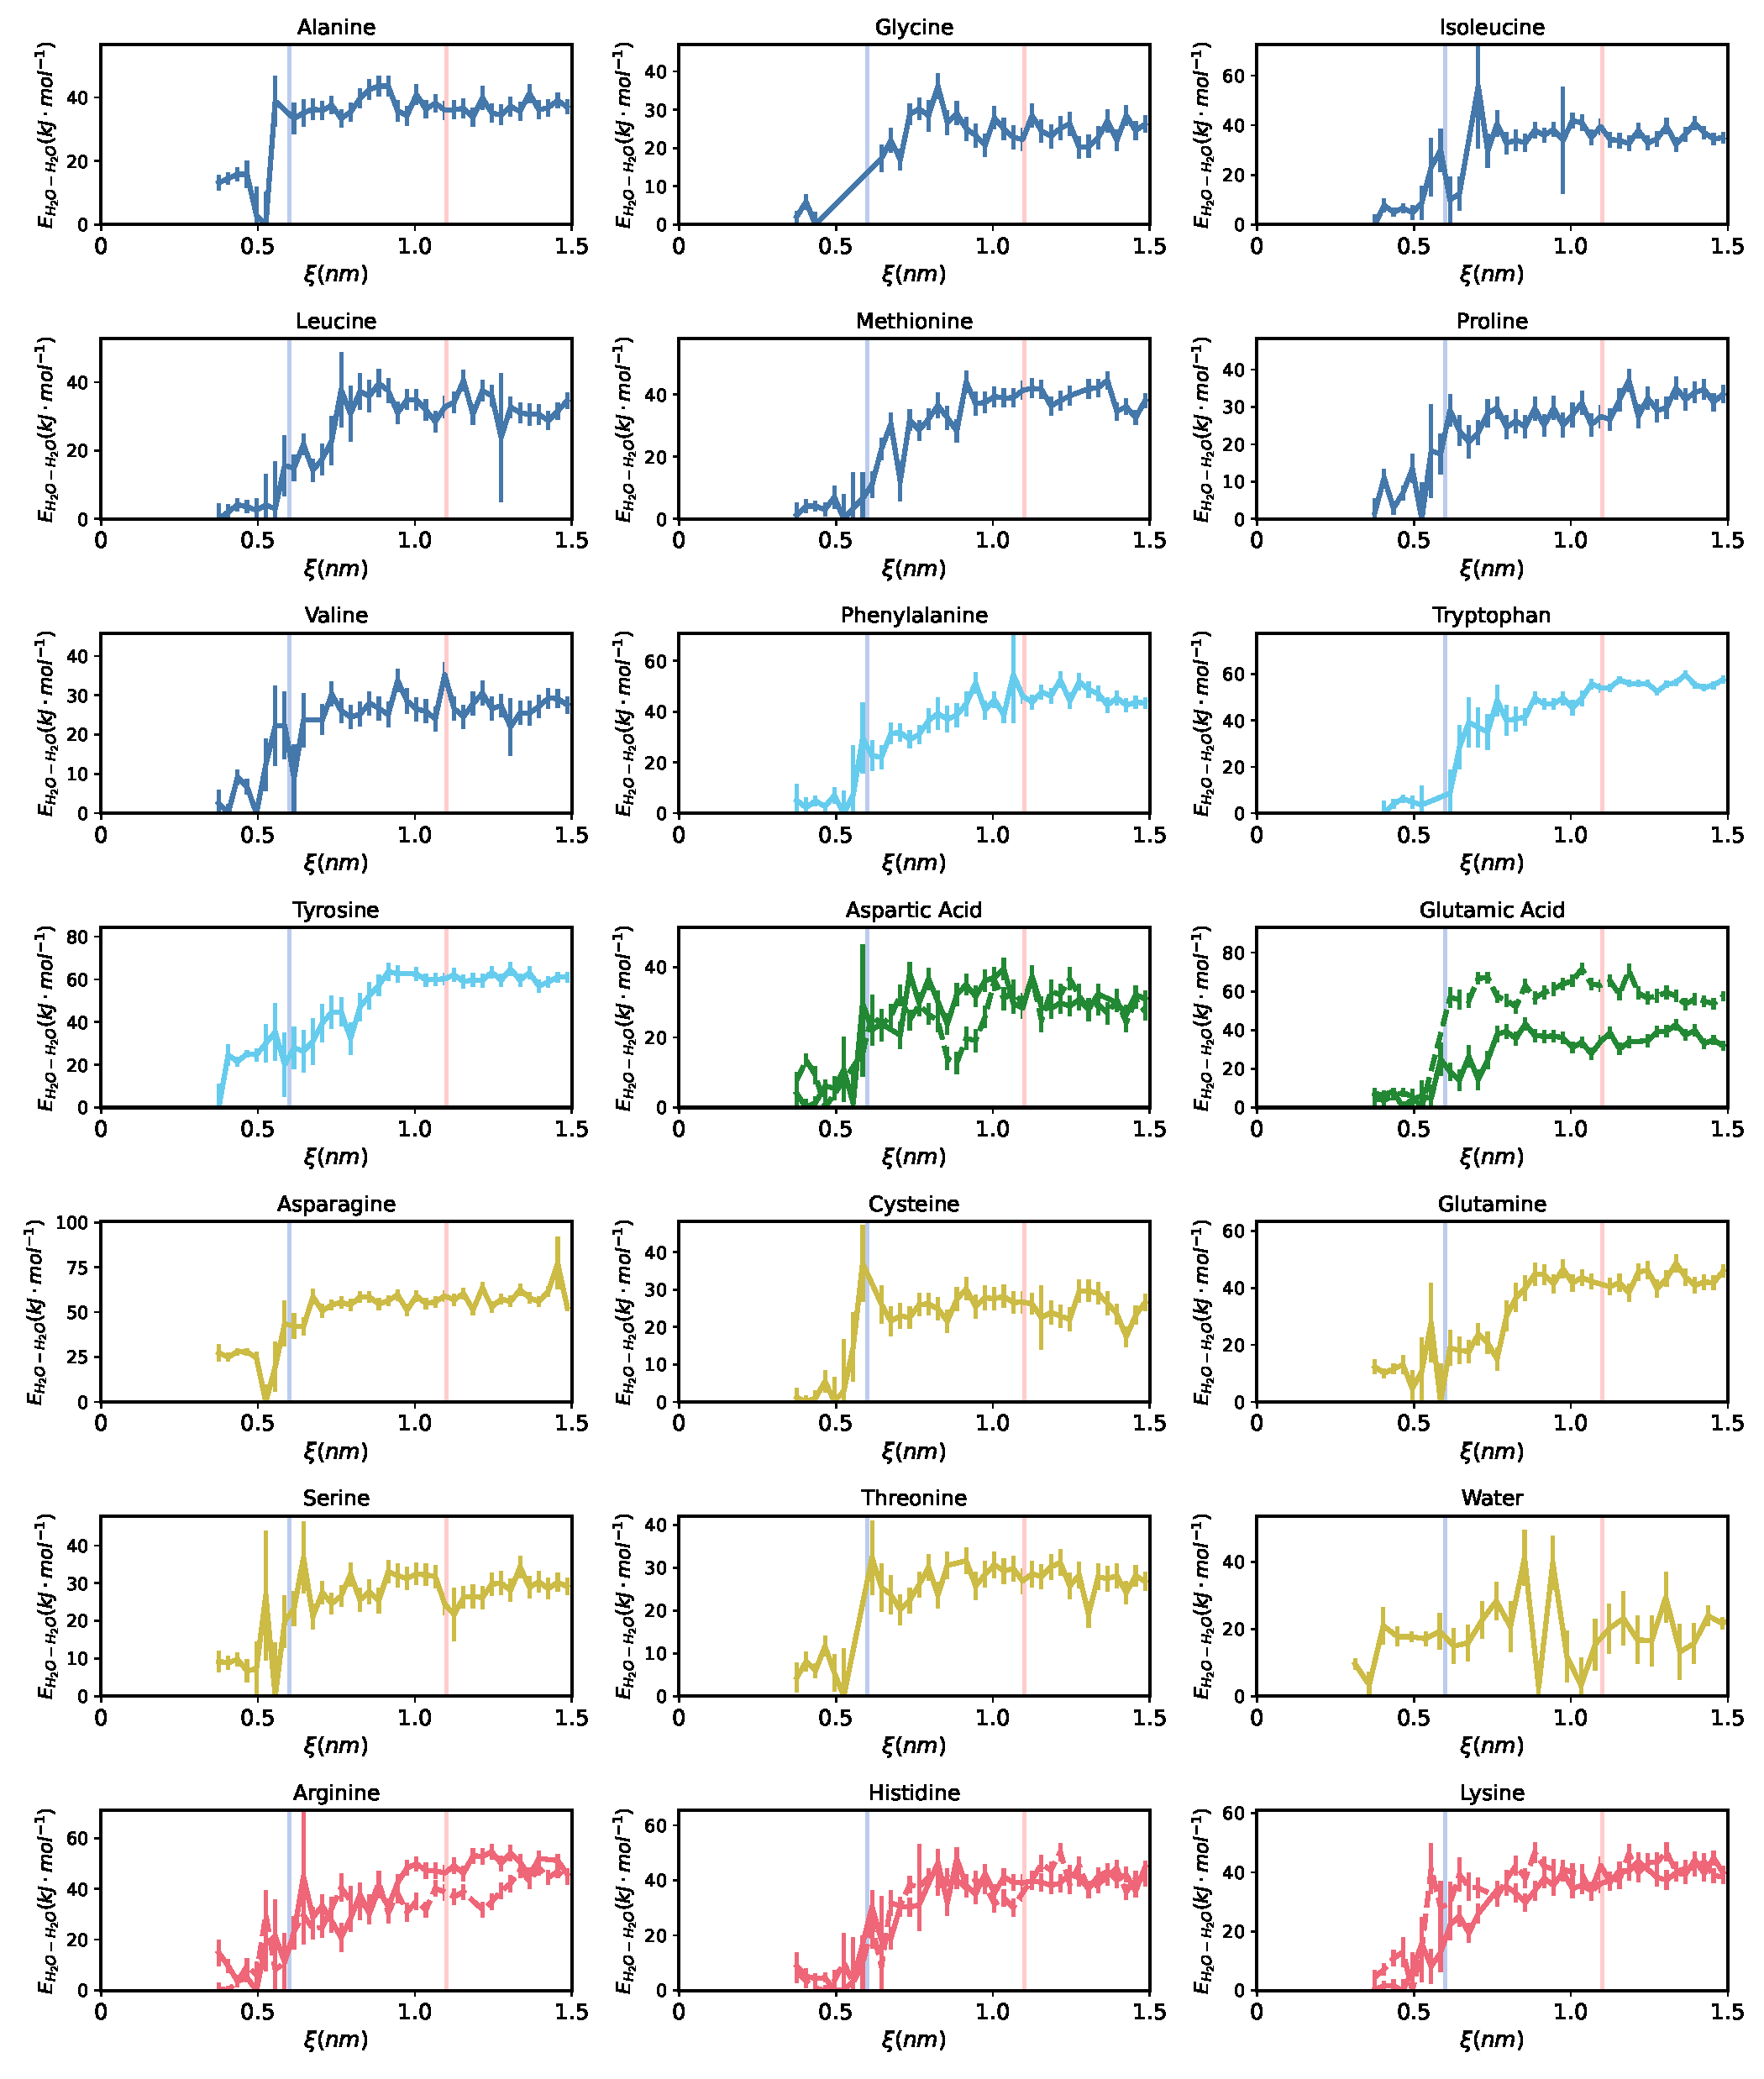
\includegraphics[width=\textwidth]{FigS7.pdf}
    \caption{Unbiased Water--Water interaction energy of the adsorption process of amino acids (or water) as a function of $\xi$ (the distance between its $\alpha$-carbon and the graphene layer, along the z-axis). Amino acids are sorted by side-chain grouping: Apolar (blue), Aromatic (Cyan), Negative (Green), Polar (Yellow), and Positive (Red). Water was grouped in with polar amino acids. For the traditionally charged amino acids (Aspartic Acid, Arginine, Glutamic Acid,  Histidine, and Lysine), both the charged and neutral forms are shown in the same panel. Charged species are depicted in a dashed line. Vertical lines are used to show the end of the "near" state (in blue) and the beginning of the "free" state (in red).}
    \label{fig:EnergyW-W}
\end{figure}

\begin{figure}[hbtp]
    \centering
    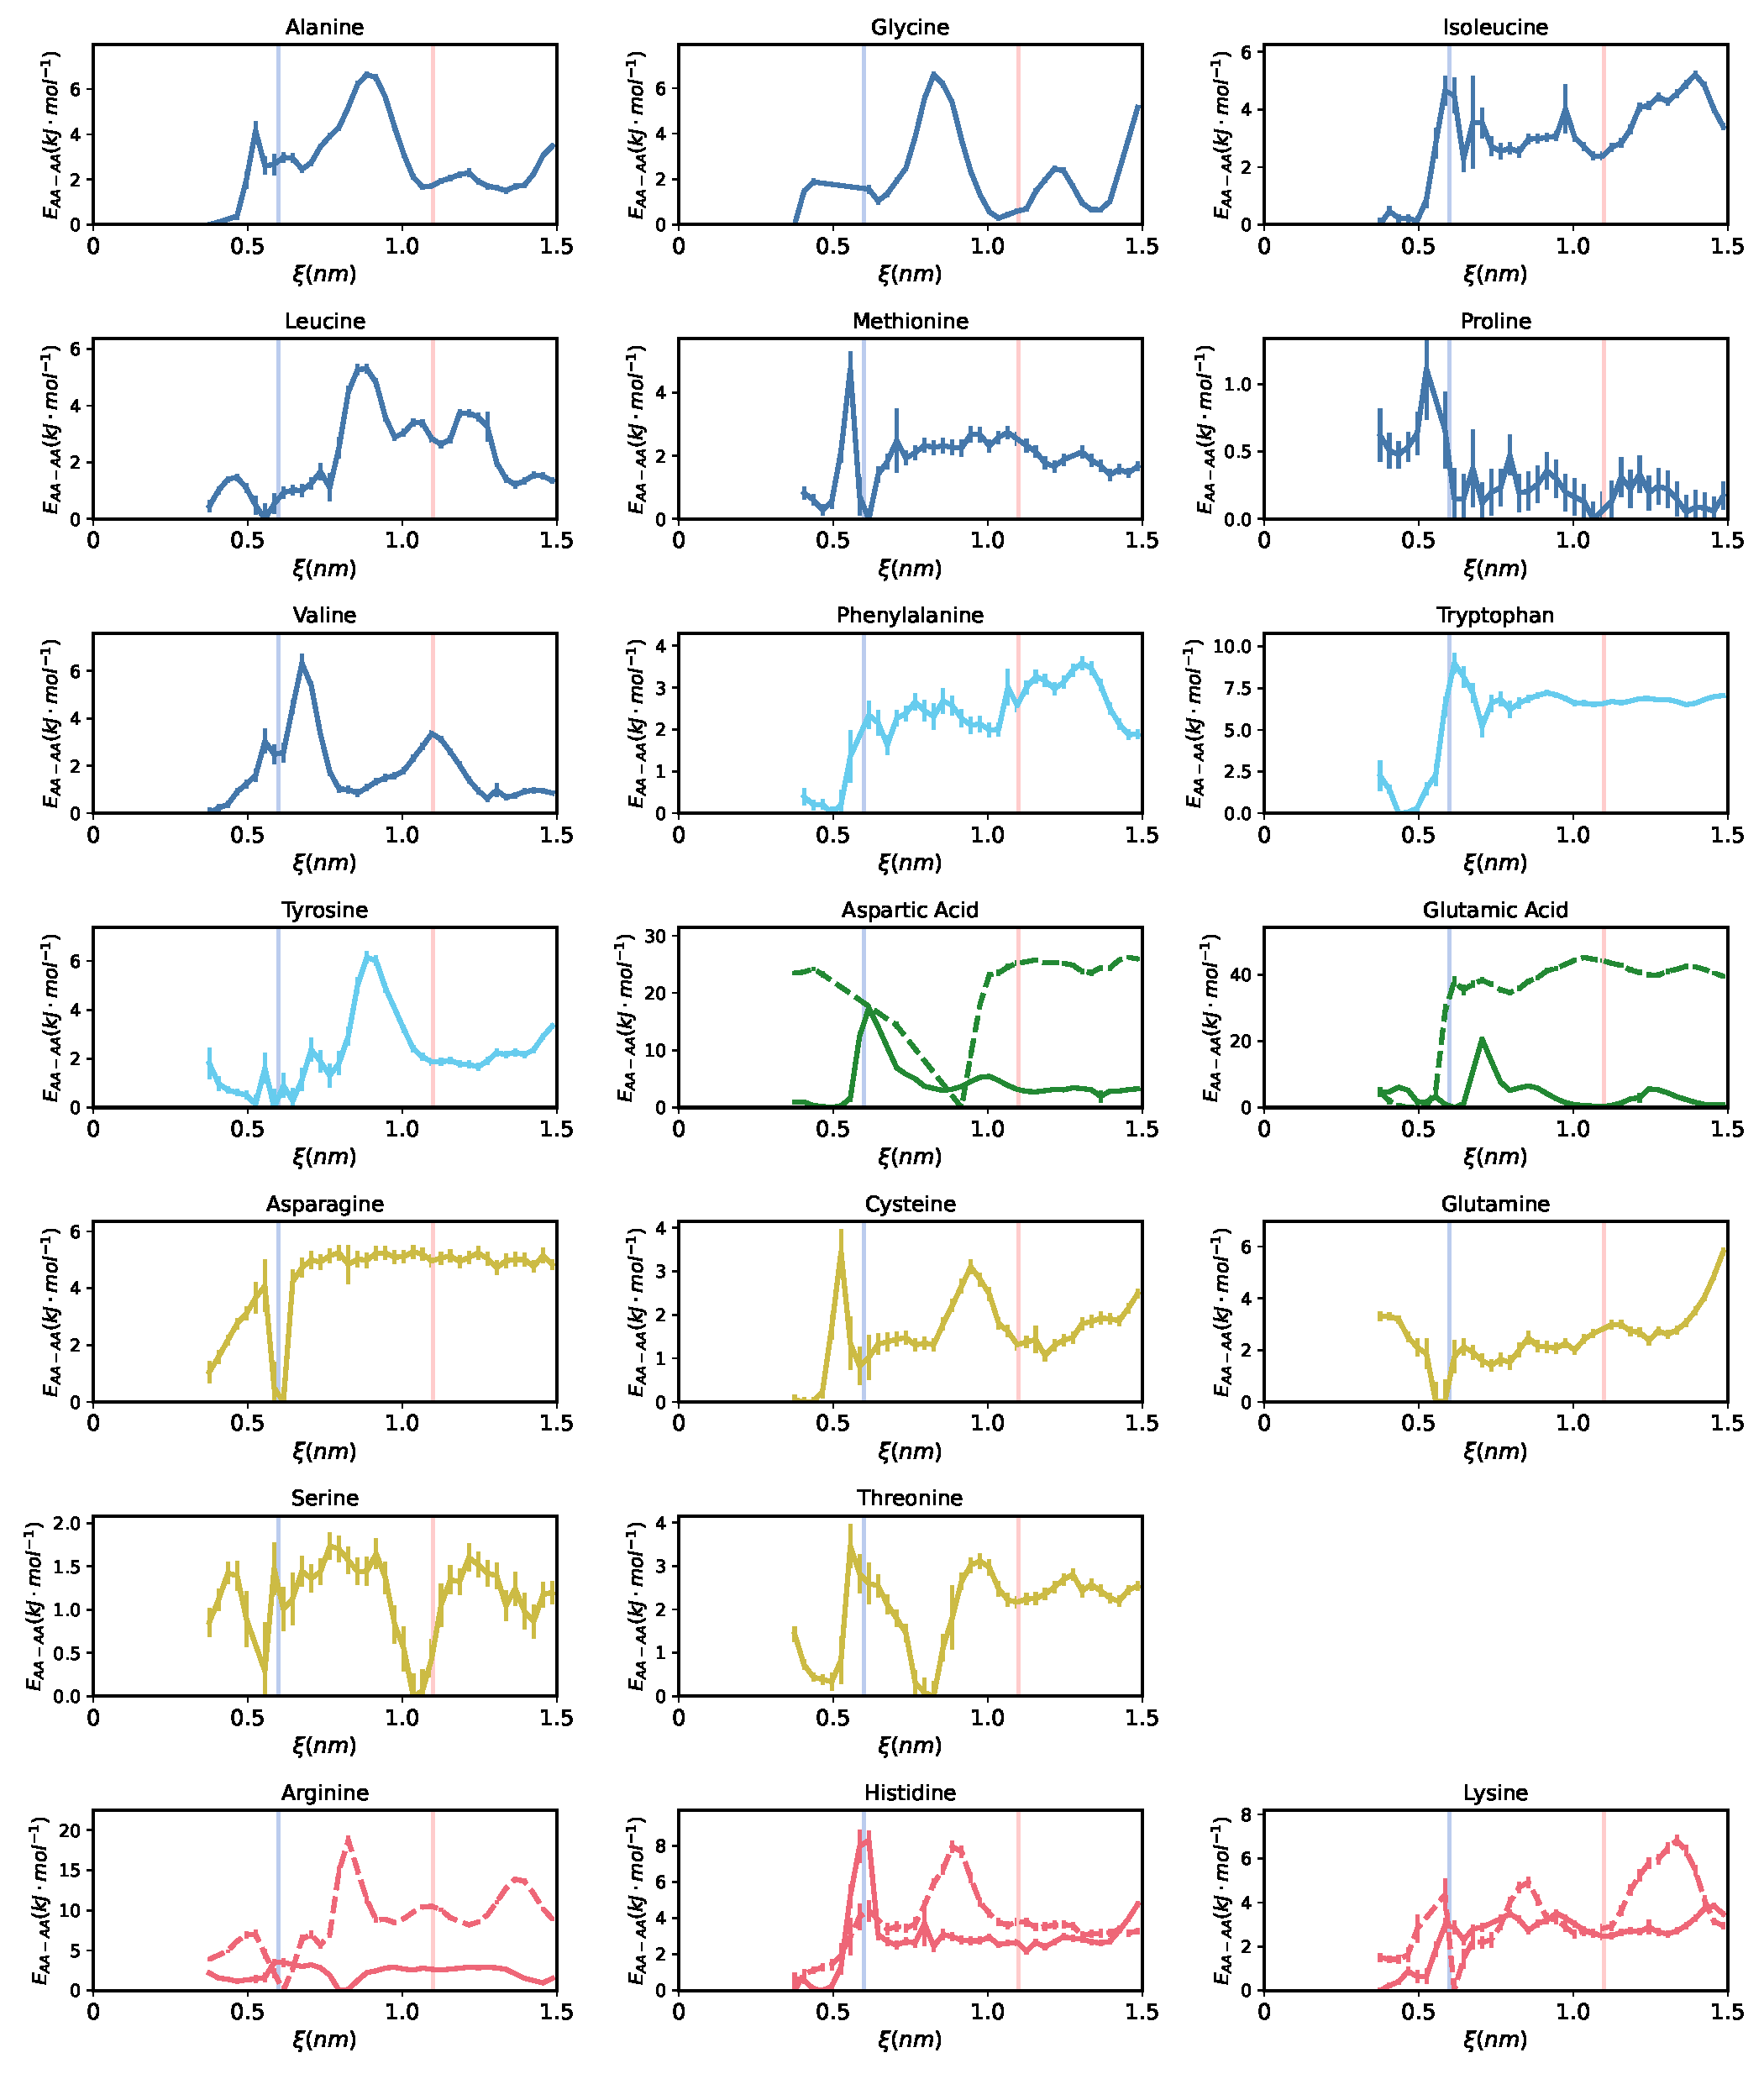
\includegraphics[width=\textwidth]{FigS8.pdf}
    \caption{Unbiased Amino-acid--Amino-acid interaction energy of the adsorption process of amino acids as a function of $\xi$ (the distance between its $\alpha$-carbon and the graphene layer, along the z-axis). Amino acids are sorted by side-chain grouping: Apolar (blue), Aromatic (Cyan), Negative (Green), Polar (Yellow), and Positive (Red). Water was grouped in with polar amino acids. For the traditionally charged amino acids (Aspartic Acid, Arginine, Glutamic Acid,  Histidine, and Lysine), both the charged and neutral forms are shown in the same panel. Charged species are depicted in a dashed line. Vertical lines are used to show the end of the "near" state (in blue) and the beginning of the "free" state (in red).}
    \label{fig:EnergyAA-AA}
\end{figure}

\newpage

\section{Linear Regressions}

\begin{figure}[hbtp]
    \centering
    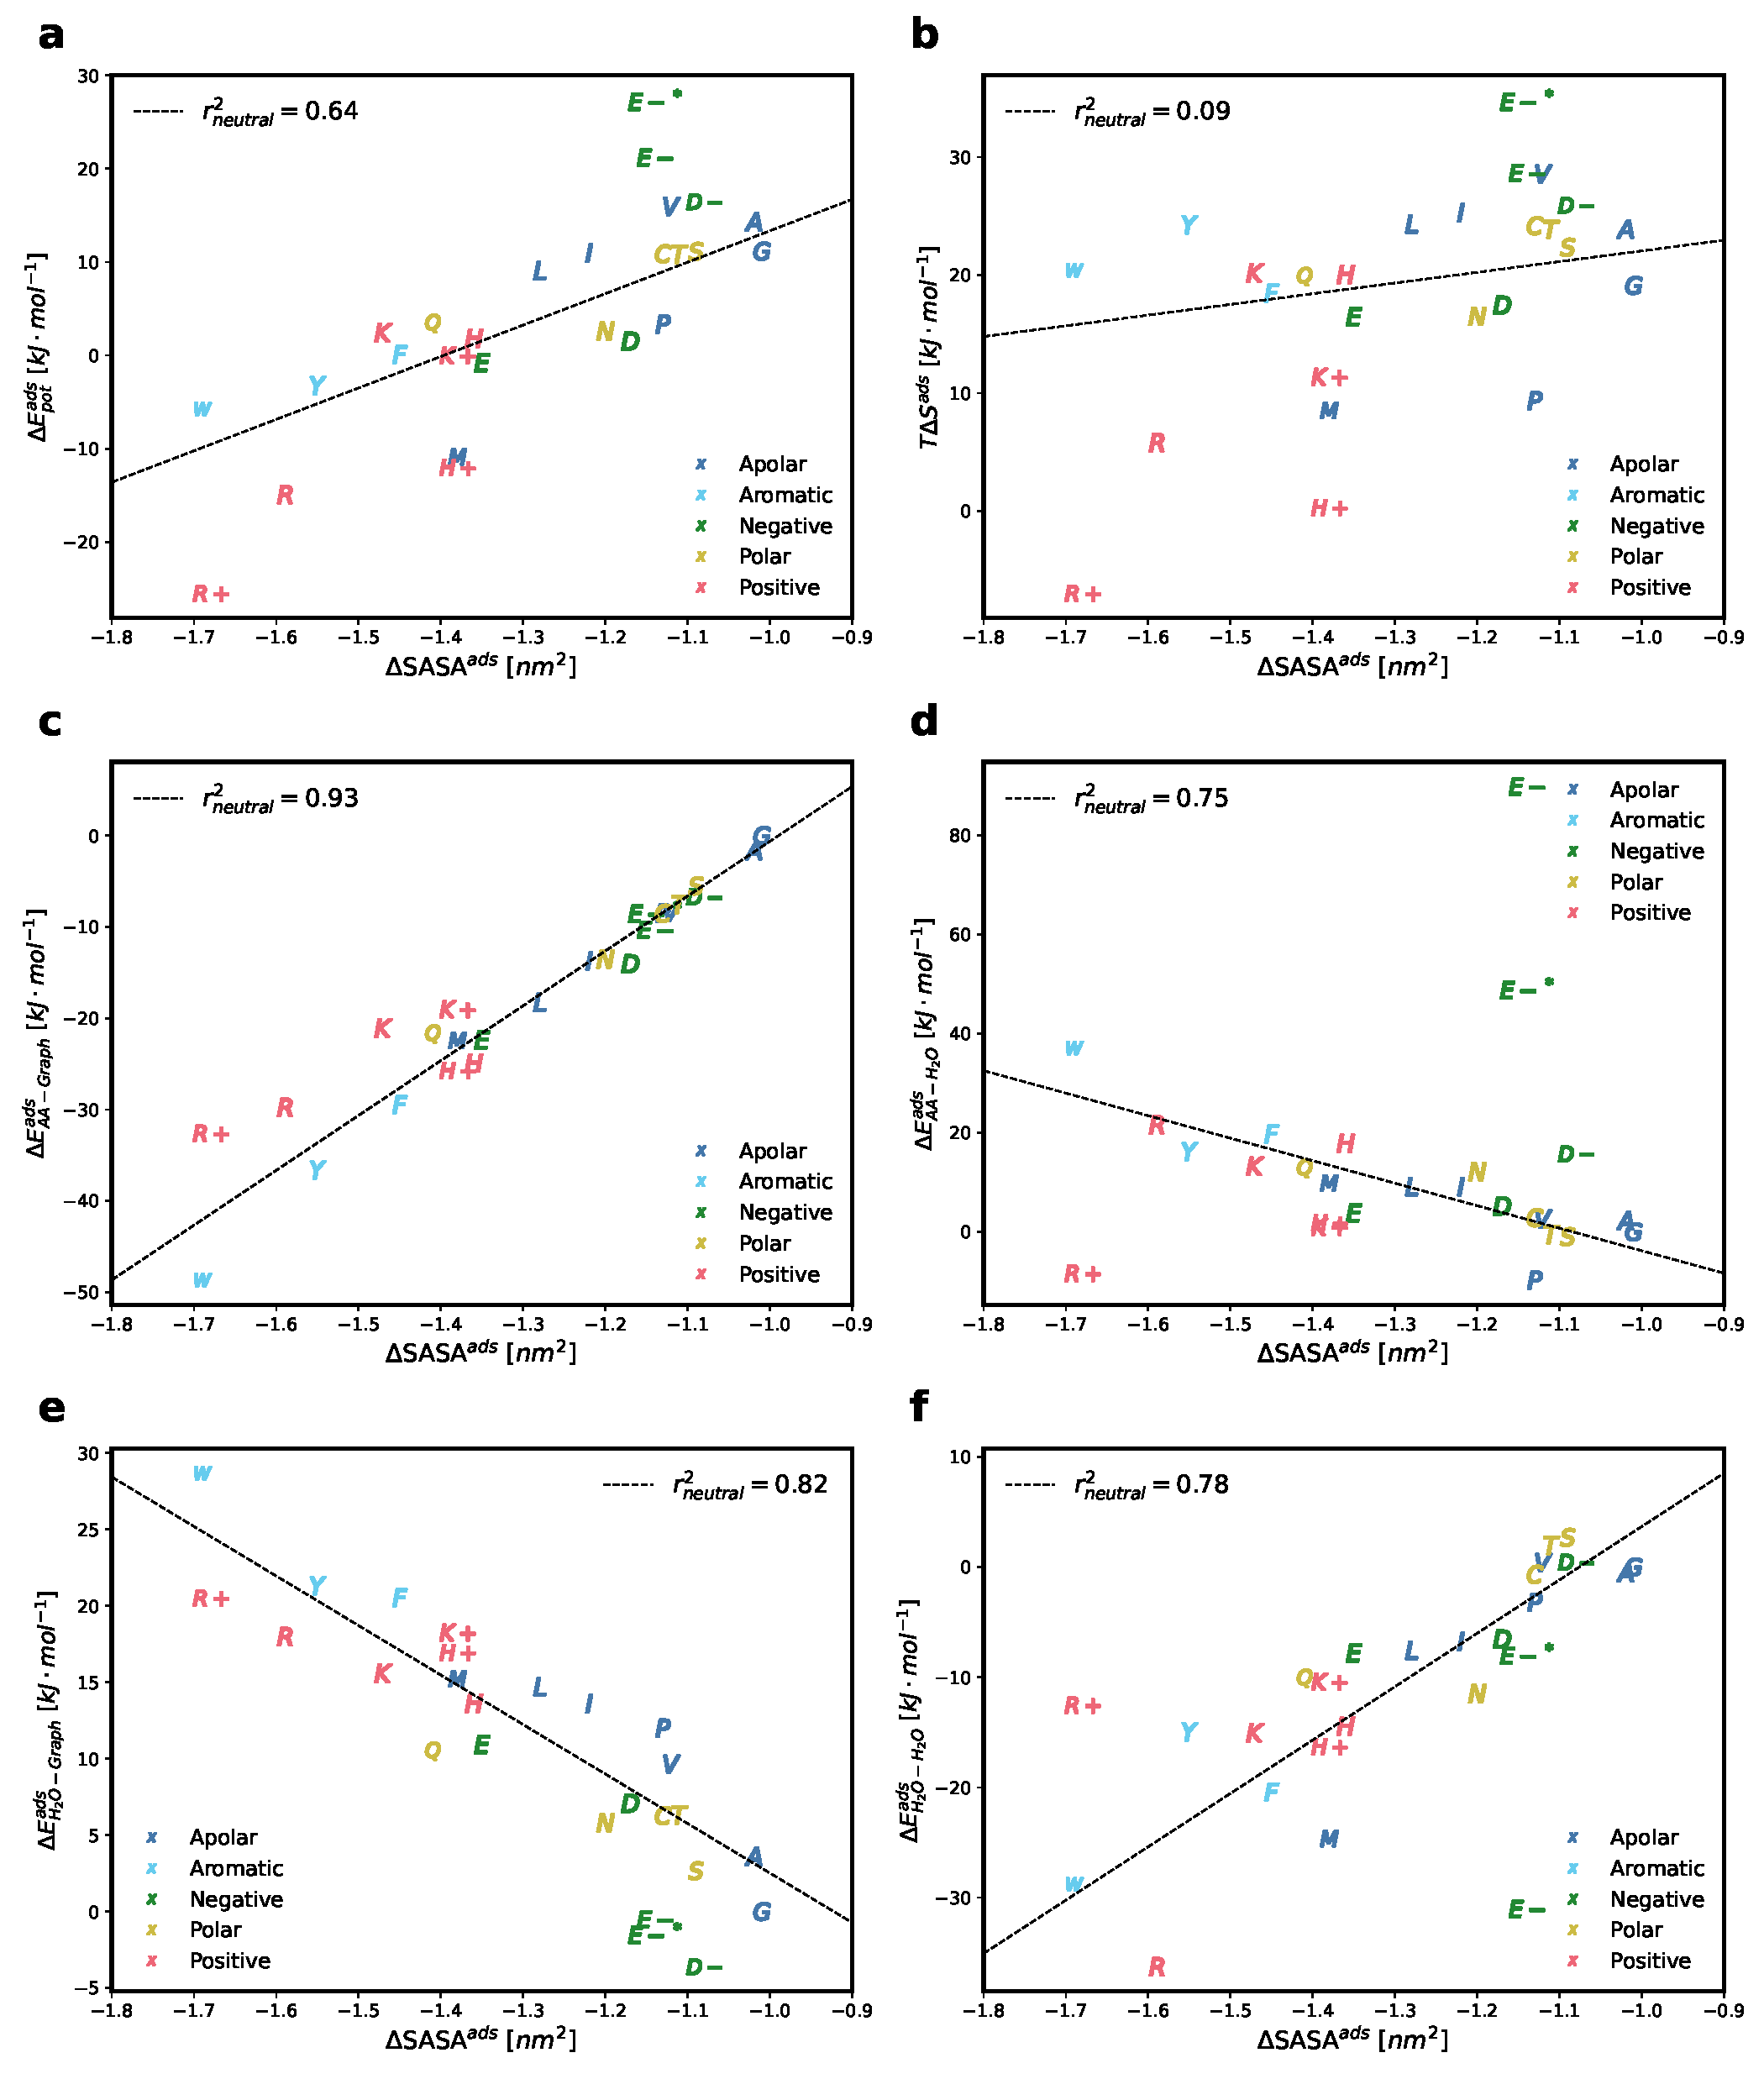
\includegraphics[width=.9\textwidth]{FigS9}
    \caption{ Energy terms correlation against $\Delta \textrm{SASA}^{ads}$. a) Potential energy of adsorption, b) Entropy (times temperature) of adsorption, c) amino-acid--graphene interaction energy of adsorption, d) amino-acid--solvent interaction energy of adsorption, e) solvent--graphene interaction energy of adsorption, e) solvent--solvent interaction energy of adsorption. In each panel a linear regression including only neutral amino acids is shown. Amino acids are shown by their single letter code, colored by side-chain grouping (Apolar in blue, Aromatic in cyan, Negative in green, Polar in yellow, and positive in red). A plus or minus sign indicates charge state, if any. For negativeglutamic acid, a value obtained by filtering out TODO-NAME configurations is shown with an asterisk.}
    \label{fig:Correlations}
\end{figure}
%\section{$\Delta A$, $\Delta E$, and $T \Delta S$ over graphene oxide}

%\begin{table}
%\centering
%\caption{\label{table:freeEnergyOxidized} Adsorption free energies ($\Delta A^{ads}$), energies ($\Delta E^{ads}$), and entropies($T \Delta S^{ads}$) for a selection of amino acids (and a water molecule) over oxidized graphene. Charged state is denoted after the amino acid's name where relevant; otherwise the amino acid was simulated in its neutral state.}
%\resizebox{\linewidth}{!}{%
%\begin{tabular}{lrrr}
%\toprule
%Name & $\Delta A^{ads}$ & $\Delta E^{ads}$ & $T \Delta S^{ads}$ \\ \hline
%Arginine (+)      & $-5.0 \pm 0.1$ & $1.1   \pm 6.4$  & $ 6.1  \pm 6.4$ \\
%Asparagine        & $-4.8 \pm 0.1$ & $-6.8  \pm 5.6$  & $-2.0  \pm 5.6$  \\
%Glutamic Acid (-) & $-6.0 \pm 0.1$ & $-21.9 \pm 4.6$  & $-15.9 \pm 4.6$  \\
%Glycine           & $-3.5 \pm 0.1$ & $0.7   \pm 4.3$  & $4.2   \pm 4.3$  \\
%Isoleucine        & $-1.9 \pm 0.1$ & $-0.5  \pm 6.1$  & $1.4   \pm 6.1$  \\
%Phenylalanine     & $2.4  \pm 0.1$ & $-5.0  \pm 8.2$  & $-7.3  \pm 8.2$  \\
%Water             & $0.5  \pm 0.1$ & $7.5   \pm 11.4$ & $7.0   \pm 11.4$  \\
%\bottomrule
%\end{tabular}
%}
%\end{table}

\newpage

\section{Stacking}
\newpage
\begin{table}
\centering
\caption{Different kinds of stacking as a percentage of simulation time spent presenting the relevant interaction. Final values are the difference between the near and free states. For tryptophan, stacking was calculated independently for the benzene (B) and pyrrole (P) ring.}
\resizebox{\linewidth}{!}{%
\begin{tabular}{lccc}
\toprule
Amino acid     & $\pi-\pi$ Stacking  & Cation$-\pi$ Stacking & Guanidinium$-\pi$ Stacking  \\
\hline
Arginine       & --                    & --                      & $52.8 \pm 1.5\%$            \\
Arginine (+)   & --                    & $96.2 \pm 1.0 \%$     & $90.0 \pm 1.0\%$            \\
Histidine      & $75.1 \pm 0.5 \%$   & --                      & --                            \\
Histidine (+)  & $83.6 \pm 0.4 \%$   & $96.6 \pm 0.2 \%$     & --                            \\
Lysine (+)     & --                    & $50.5 \pm 0.5 \%$     &     --                     \\
Phenylalanine  & $73.7 \pm 0.5 \%$   & --                      & --                            \\
Tryptophan (B) & $96.3 \pm 0.2 \%$ & --                      & --                            \\
Tryptophan (P) & $96.1 \pm 0.2\%$    & --                      & --                            \\
Tyrosine       & $92.7 \pm 0.2 \%$   & --                      & --                            \\
\bottomrule
\end{tabular}
}
\end{table}
\newpage
\section{Comparisons with reported $\Delta A^{ads}$}

\begin{figure}
    \centering
    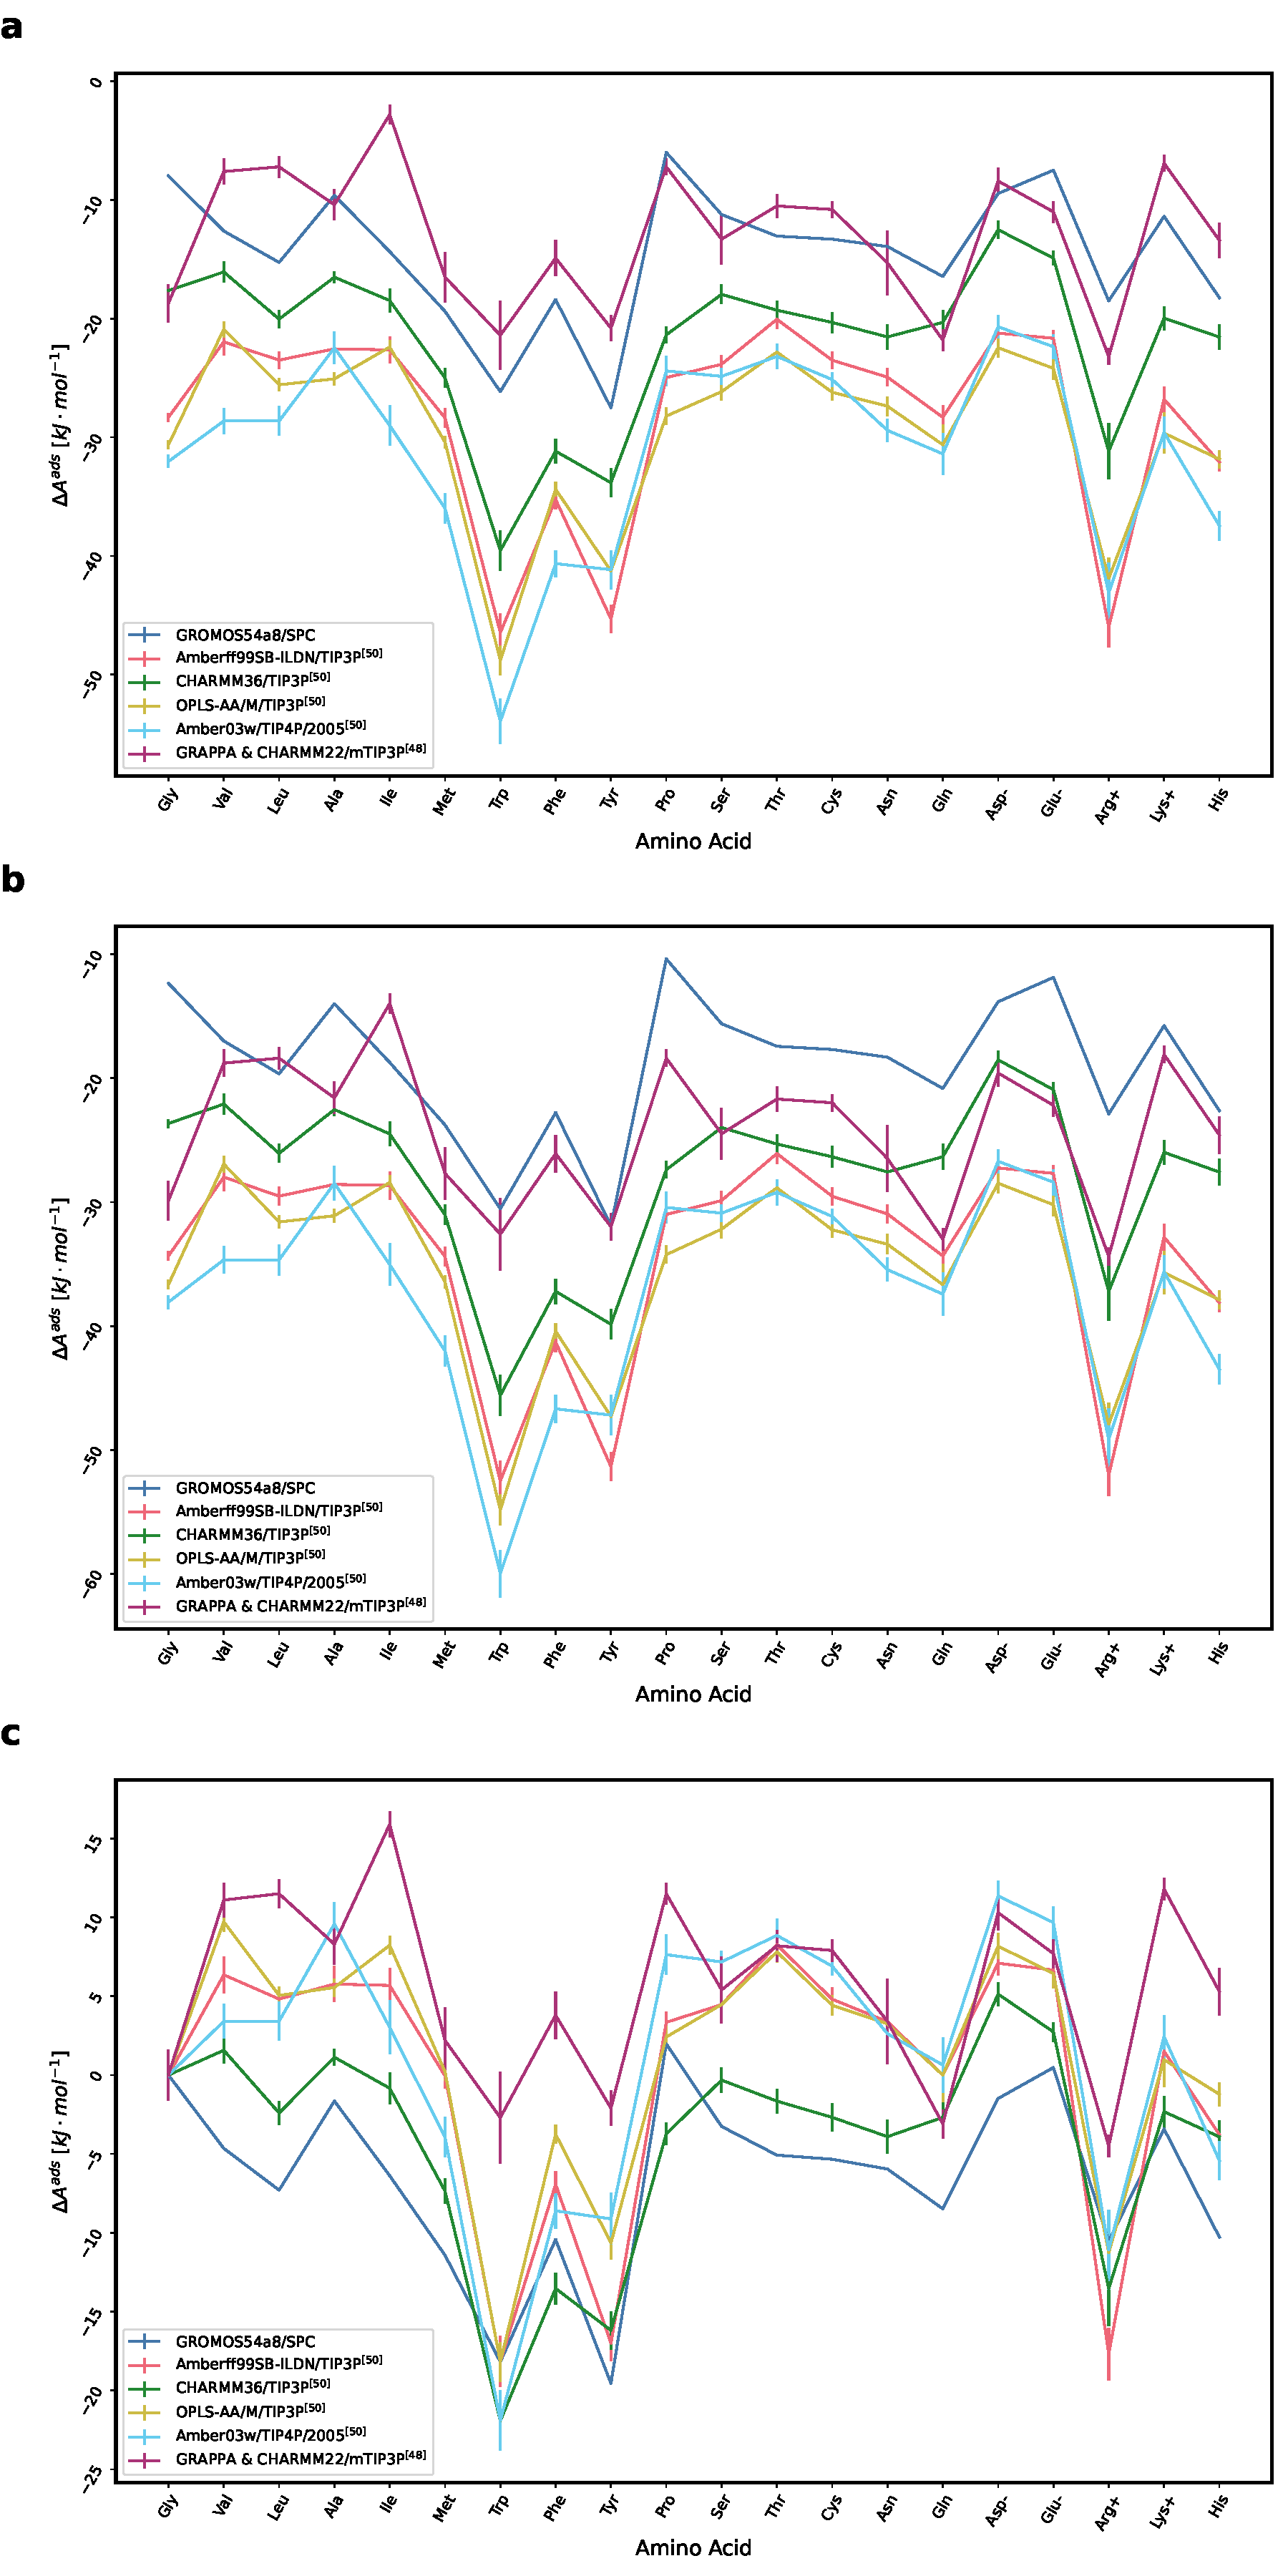
\includegraphics[width=.6\textwidth]{figures/FigS10.pdf}
    \caption{Comparisons of calculated values (GROMOS54A8) to values reported by Dasetty et al. (Amberff99SB-ILDN, CHARMM36, OPLS-AA/M, and Amber03w) and by Hughes \& Walsh (GRAPPA \& CHARM22). a) Uncorrected values. b) Corrected values by the standard state. c) Values reduced by the $\Delta A^{ads}$ of Glycine.}
    \label{fig:Comparisons}
\end{figure}

\end{document}
